%%%%%%%%%%%%%%%%%%%%%%%%%%%%%%%%%%%%%%%%%%%%%%%%%%%%%%%%%%%%%%%
\section{Jets}\label{sec:jets}
%%%%%%%%%%%%%%%%%%%%%%%%%%%%%%%%%%%%%%%%%%%%%%%%%%%%%%%%%%%%%%%

Quarks and gluons produced in the high-energy processes
such as hard scattering of partons in pp collisions, carry a color charge and 
%Particles carrying a color charge, such as quarks,
cannot exist in free form because of QCD confinement which only allows for colorless states (Section~\ref{subsec:QCD}).
%Quarks and gluons interact with pairs of quarks and anti-quarks produced from the vacuum until the formation of stable colourless hadrons.
At detector level, only the ensemble of the final colourless stable hadrons, simulated by the parton shower algorithms, can be observed.
This exhibits as a jet of collimated particles which reflects the energy and the flight direction of the initial parton.
Therefore, a jet is a cluster of charged particle tracks and calorimetric energy deposits in the detector, whose properties depend on the algorithm used for its definition.
%The ensemble of the final colourless objects is called a \textit{jet} and it is reconstructed in the detector from energy depositions and charged particle momenta.
%The jets point back to the primary interaction, i.e. to the partons the jets originated from, but a correction for hadronization and detector effects is needed.
The jet-clustering algorithms cluster particles (at parton, particle or detector level) into jets and reconstruct the energy and direction of the original parton. The task of a jet-clustering algorithm is to allow comparisons between theoretical predictions, which are usually described by perturbative calculations, and experimental data. This is achieved by reducing the complex structure of particle jets from a scattered parton to a simple four-momentum, which represents the main property of particle jets.
In order to guarantee a meaningful calculation of theory predictions, jet-clustering algorithms are characterized by two important properties.
%Two properties of jet clustering algorithms are desired to be able to calculate meaningful theory predictions.
Clustering algorithms need to be infrared-safe, which means that the emission of infinitesimally-low-energy partons from partons inside a jet does not affect the jet properties. Furthermore, they need to be collinear-safe, which means that jet properties are not affected by the splitting of a parton inside a jet into two collinear partons.
Jet algorithms for hadron colliders can be divided into two classes: cone~\cite{Salam:2007xv} and sequential clustering~\cite{Catani:1993hr,Ellis:1993tq,Dokshitzer:1997in,Wobisch:1998wt,Cacciari:2008gp} algorithms.
%Jet algorithms for hadron colliders can be divided into two classes. One possibility is based on proximity in coordinate space, cone jet algorithms [180, 181]) whereas the other uses proximity in momentum space by successively merging pairs of particles in order of increasing relative transverse momentum, kT algorithms [182, 183]). For this work only the anti-kT algorithm of the kT family is used and detailed in the following.
The main algorithms used by LHC experiments belong to the second class and are the anti-$k_t$~\cite{Cacciari:2008gp} (AK) and the Cambridge--Aachen (CA)~\cite{Catani:1993hr,Dokshitzer:1997in} algorithms. In fact, they are found to fulfill theoretical requirements and to exhibit good properties for experimental measurements. For this work both algorithms are used and described in the following.
 
 %%%%%%%% 
\subsection{Jet-clustering algorithms}\label{subsec:jetsalgo}
%%%%%%%%

In sequential jet-clustering algorithms, jets are defined through sequential, iterative procedures that combine four-vectors of input pairs of particles until certain criteria are satisfied and jets are formed. In particular, for each pair of particles $i$ and $j$, a distance variable between the two particles ($d_{ij}$), and the so-called ``beam distance'' for each particle ($d_{iB}$), are computed:
 
\begin{equation}\label{eqn:jetalgo}
d_{ij} = \mathrm{min}(p_{Ti}^{2n},p_{Tj}^{2n})\frac{\Delta R^2_{ij}}{R^2}\quad,\quad\quad\quad
d_{iB} = p_{Ti}^{2n}\quad,
\end{equation} 

\noindent where $p_{Ti}$ and $p_{Tj}$ are the transverse momenta of particles $i$ and $j$, respectively, ``min'' refers to the smaller of the two \pt values, the integer $n$ depends on the specific jet algorithm, $\Delta R^2_{ij}$ is the distance between $i$ and $j$ in the $\eta$-$\phi$ plane, and $R$ is a free distance parameter, with all angles expressed in radians. The particle pair ($i$, $j$) with smallest $d_{ij}$ is combined into a single object. All distances are recalculated using the new object, and the procedure is repeated until, for a given object $i$, all the $d_{ij}$ are greater than $d_{iB}$. Object $i$ is then classified as a jet and not considered further in the algorithm. The process is repeated until all input particles are clustered into jets.

The distance parameter $R$ is responsible for defining the angular size of the jet. The parameter $n$ governs the topological properties of the jets and, depending on its value, three different classes of clustering algorithms are distinguished. For $n = 1$ the procedure is referred to as the $k_t$ algorithm (KT)~\cite{Cacciari:2008gp}, which clusters soft objects before harder ones are added to the final jet, mimicking in reverse the parton fragmentation and gluon emission processes. For this reason, the algorithm tends to construct jets of irregular shapes which depend on the detailed distribution of soft particles in an event.
In addition, they are sensitive to the presence of low-\pt pileup contributions.
%The KT jets tend to have irregular shapes and are especially useful for reconstructing jets of lower momentum. For this reason, they are also sensitive to the presence of low-\pt pileup contributions.
%, and are used to compute the mean \pt per unit area of an event.
For $n = 0$, the procedure corresponds to the CA algorithm. This relies only on angular information, and, like the KT algorithm, provides irregularly-shaped jets. The CA and KT algorithms are useful in identifying jet substructure as described in Chapter~\ref{ch:vtagging}.
%The C-A algorithm still reflects aspects of the QCD parton shower, in particular the angular ordering of emissions. However, it is less directly relatedtothestructureofQCDpartonsplittingfunctionsthanthekT algorithmis,and represents a compromise between reflecting the structure of the parton shower and maintaining some insensitivity to soft radiation.
For $n = -1$, the procedure corresponds to the AK algorithm, which compares the inverse square of the transverse momenta.
The AK algorithm is used extensively in LHC experiments and by the theoretical community for finding well-separated jets. The use of the inverse square of the \pt as a weight in the $d_{ij}$ distances has the advantage that hard objects collect adjacent soft ones before these are clustered among themselves into harder object. %This means that the most energetic cores of jets are found first.
%, figuratively reproducing in reverse the parton fragmentation and gluon emission processes. --> not true! harder objects come first in QCD splitting.
This property makes the algorithm independent on soft radiation, preserving infrared-safety. Low-energy gluons emitted at large angles are picked up by the algorithm rather late in the clustering process and therefore do not affect the jet properties. They are picked up after all hard emissions at small angles and before two soft particles can cluster with each other. Soft emissions will therefore not cluster into separate jets, preserving infrared-safety. The AK algorithm is also collinear-safe as the clustering is driven by the angular distance between two particles. Furthermore, as soft particles clustered later have a minimal impact on the larger four-momentum of the jet core, the AK algorithm tends to cluster particles out to distances $R$ from the core of a jet, yielding very regular jets. This allows for straight-forward calibration and understanding of the detector acceptance. The behaviours of the CA and AK jet algorithms are illustrated in Fig.~\ref{fig:jetalgos}. 
%this algorithm tends, by construction, to form almost circular jets allowing for straight-forward calibration and understanding of the detector acceptance. The behaviours of the CA and AK jet algorithms are illustrated in Fig.~\ref{fig:jetalgos}. 
%As soft particles clustered later have a minimal impact on the larger four-momentum of the jet core, the anti-kT algorithm tends to cluster particles out to distances R from the core of a jet, yielding very regular jets.
%This algorithm is collinear-safe as the clustering is driven by the angular distance between two particles. Gluons emitted at small angles are picked up by the algorithm in early steps of the iteration and therefore do not affect the jet properties. The algorithm is also infrared-safe. Due to the weighting with the inverse maximum squared transverse momentum, the emission of additional low energy gluons are picked up rather late in the clustering process. They are picked up after all hard emissions at small angles, but, importantly, before two soft particles can cluster with each other. Soft emissions will therefore not cluster into separate jets, preserving infrared-safety.
%The AK algorithm has very good experimental properties. By construction it tends to form almost circular jets with a radius of R. This is demonstrated for an example event in Fig. 7.1. Only if two jets are closer than 2R, the shape of the two jets varies from being circular. Experimentally this feature is very important as it allows straight-forward calibration and un- derstanding of the detector acceptance. Due to its limited cone size, the measurement of jets can be restricted to active detector regions. Due to the fixed cone size, the number of detector cells to be clustered into a jet is constant over certain detector regions and therefore straight-forward to calibrate.

\begin{figure}[!htb]
\centering
\subfigure[]{\label{fig:jetalgos_a}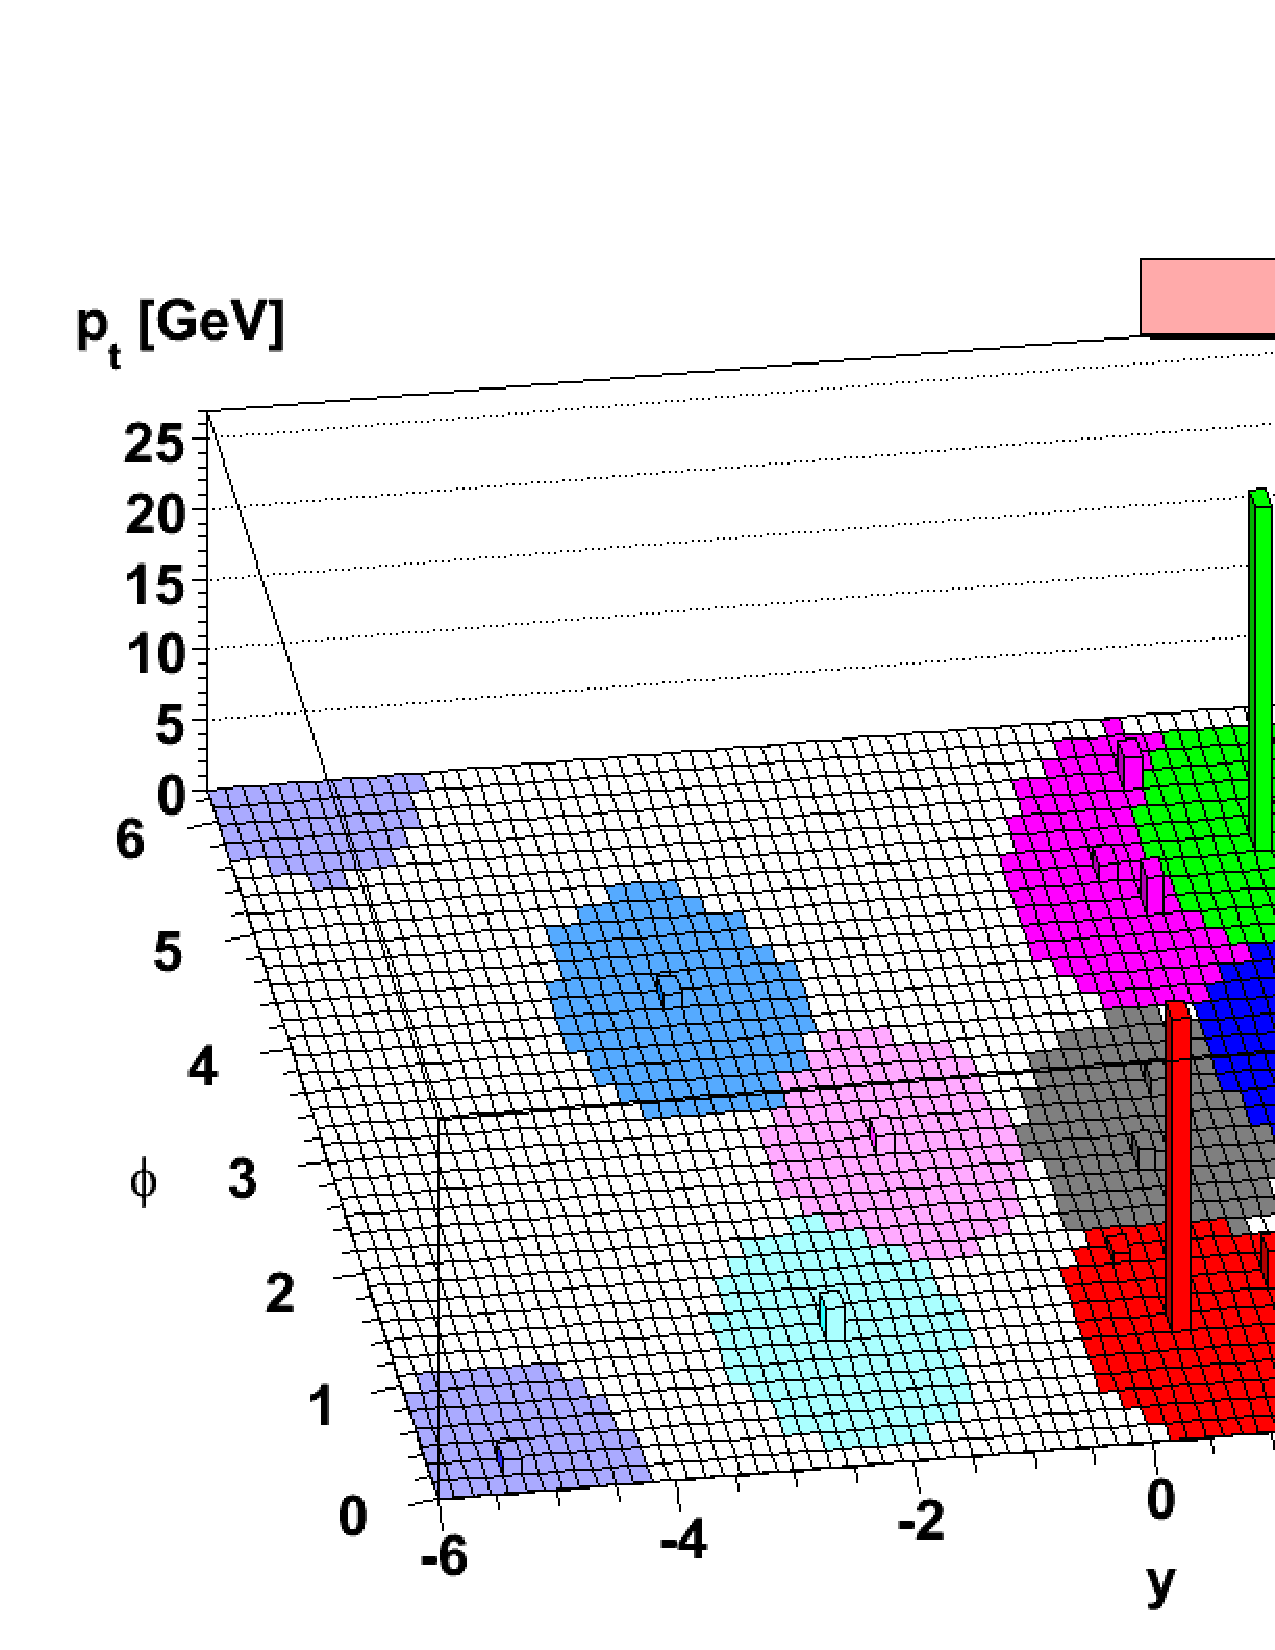
\includegraphics[width=0.45\textwidth]{\chsix/herwig-parton-level-ev-antikt-R1p0-ghosted4root.pdf}}
\subfigure[]{\label{fig:jetalgos_b}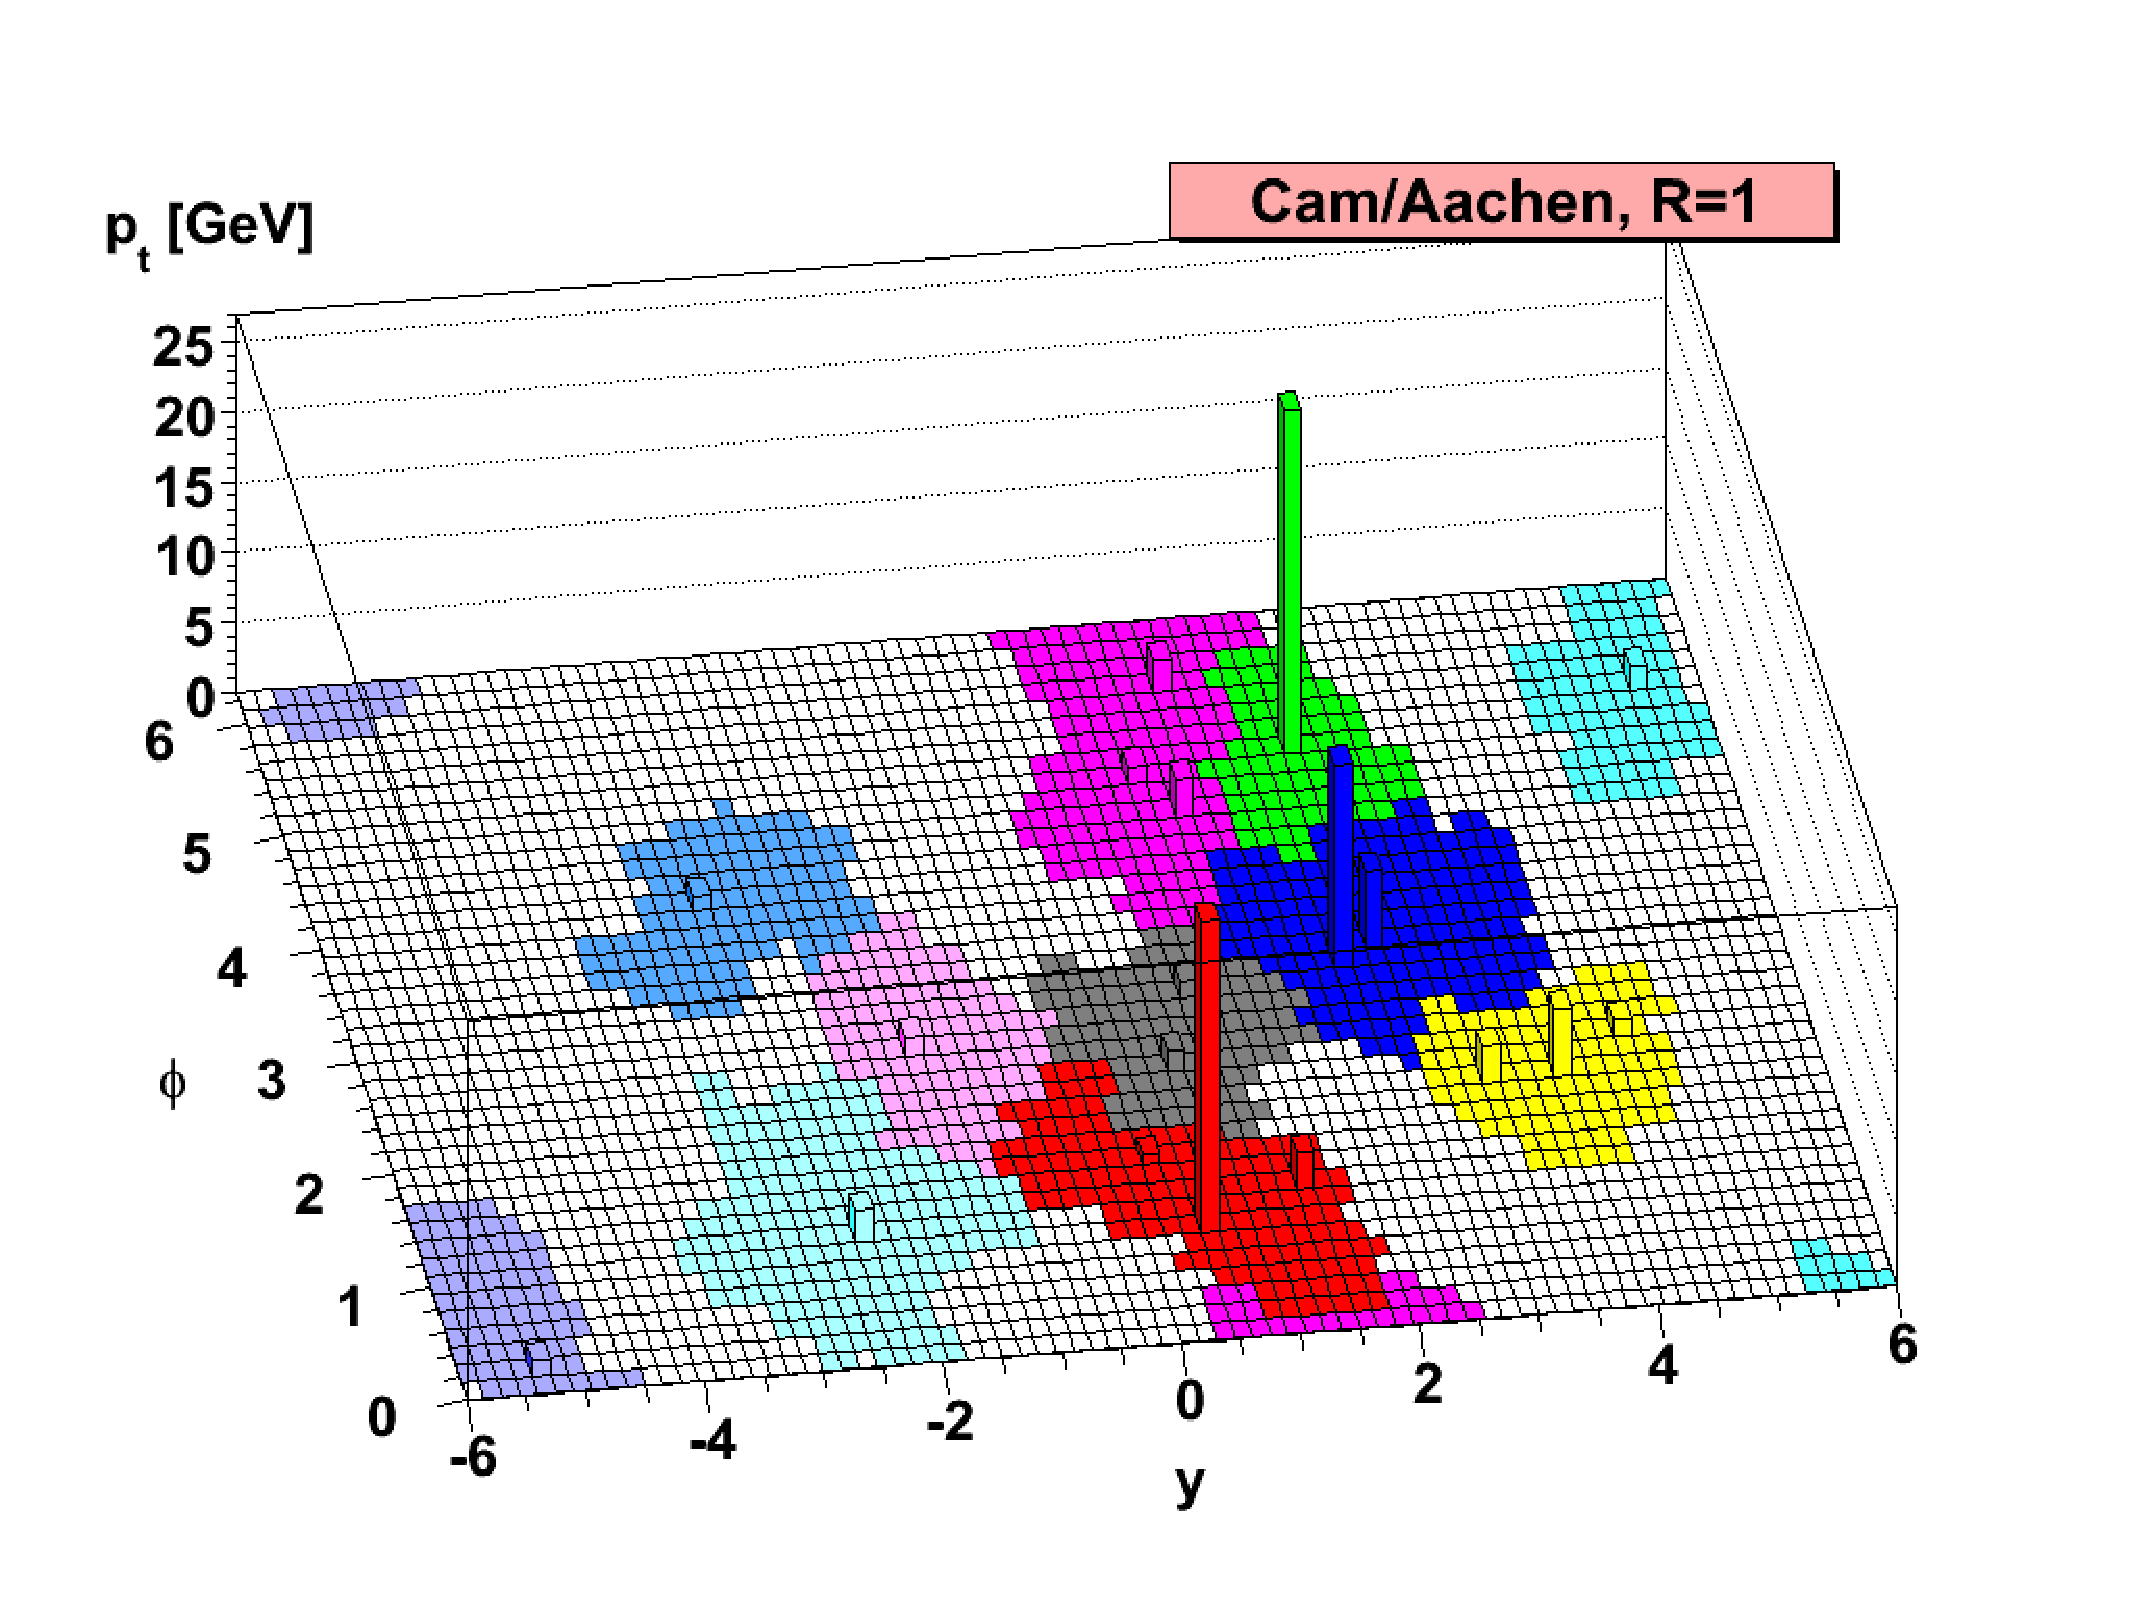
\includegraphics[width=0.45\textwidth]{\chsix/herwig-parton-level-ev-cam-R1p0-ghosted4root.pdf}}
\caption{An example of jet-clustering with the AK (a) and CA (b) algorithms. The reconstructed jets are shown as colored regions~\cite{Cacciari:2008gp}.}
\label{fig:jetalgos}
\end{figure}

The choice of the distance parameter $R$ generally depends on the analysis. While large cone-size jets collect all energy from the scattered parton, they also pick up a large contribution of background energy from the underlying event or pileup interactions. Small cone-size jets pick up little contamination, but may not collect all energy from the scattered parton. 
The default choice in CMS for physics analyses in Run~1 and Run~2 uses the AK algorithm with $R = 0.5$ (AK5) and $R = 0.4$ (AK4), respectively, since more collimated jets are expected at higher $\sqrt{s}$. The AK5 or AK4 algorithms are used in this analysis to put requirements on additional b jets in the event selection (Section~\ref{sec:finalselection}), along with the b-tagging algorithm described in Section~\ref{subsec:bjets}.

A larger value of $R$ increases the efficiency to entirely reconstruct the highly energetic products in the decays into hadrons of boosted V and Higgs bosons.
In fact, the average angular distance between the decay products is inversely proportional to the \pt of the mother particle. The default choice in CMS for physics analyses involving boosted V or Higgs bosons decaying hadronically is $R = 0.8$. In particular, CA8 and AK8 jets are used for Run~1 and Run~2 data analyses, respectively. The chosen value of $R$ provides a high efficiency for V or Higgs bosons with small boost and ensures that no efficiency is lost in the transition from the classical reconstruction in two small jets at low boson \pt to the reconstruction as a single large-cone jet at higher values. Another point to consider when choosing the value of $R$ is the \ttbar data sample available for validating highly boosted W jets (Section~\ref{sec:vtagging}). If $R$ is chosen too large, the b quark from the $\cPqt\to\PW\cPqb$ decay tends to merge into the W jet. The chosen value of $R$ is the result of a compromise between high efficiency for V or Higgs bosons with small boost and a sufficiently large sample of W jets in \ttbar data for validating the boosted boson jet identification procedure. Figure~\ref{fig:ca8effVsPt} shows the \pt range of W bosons for which the CA8 algorithm is efficient and compares this to the efficiency for reconstructing W bosons from two AK5 jets. Above a \pt of 200\GeV, the CA8 jet algorithm, used to identify W jets, becomes more efficient than the reconstruction of a W boson from two AK5 jets.

\begin{figure}[!htb]
 \begin{center}
  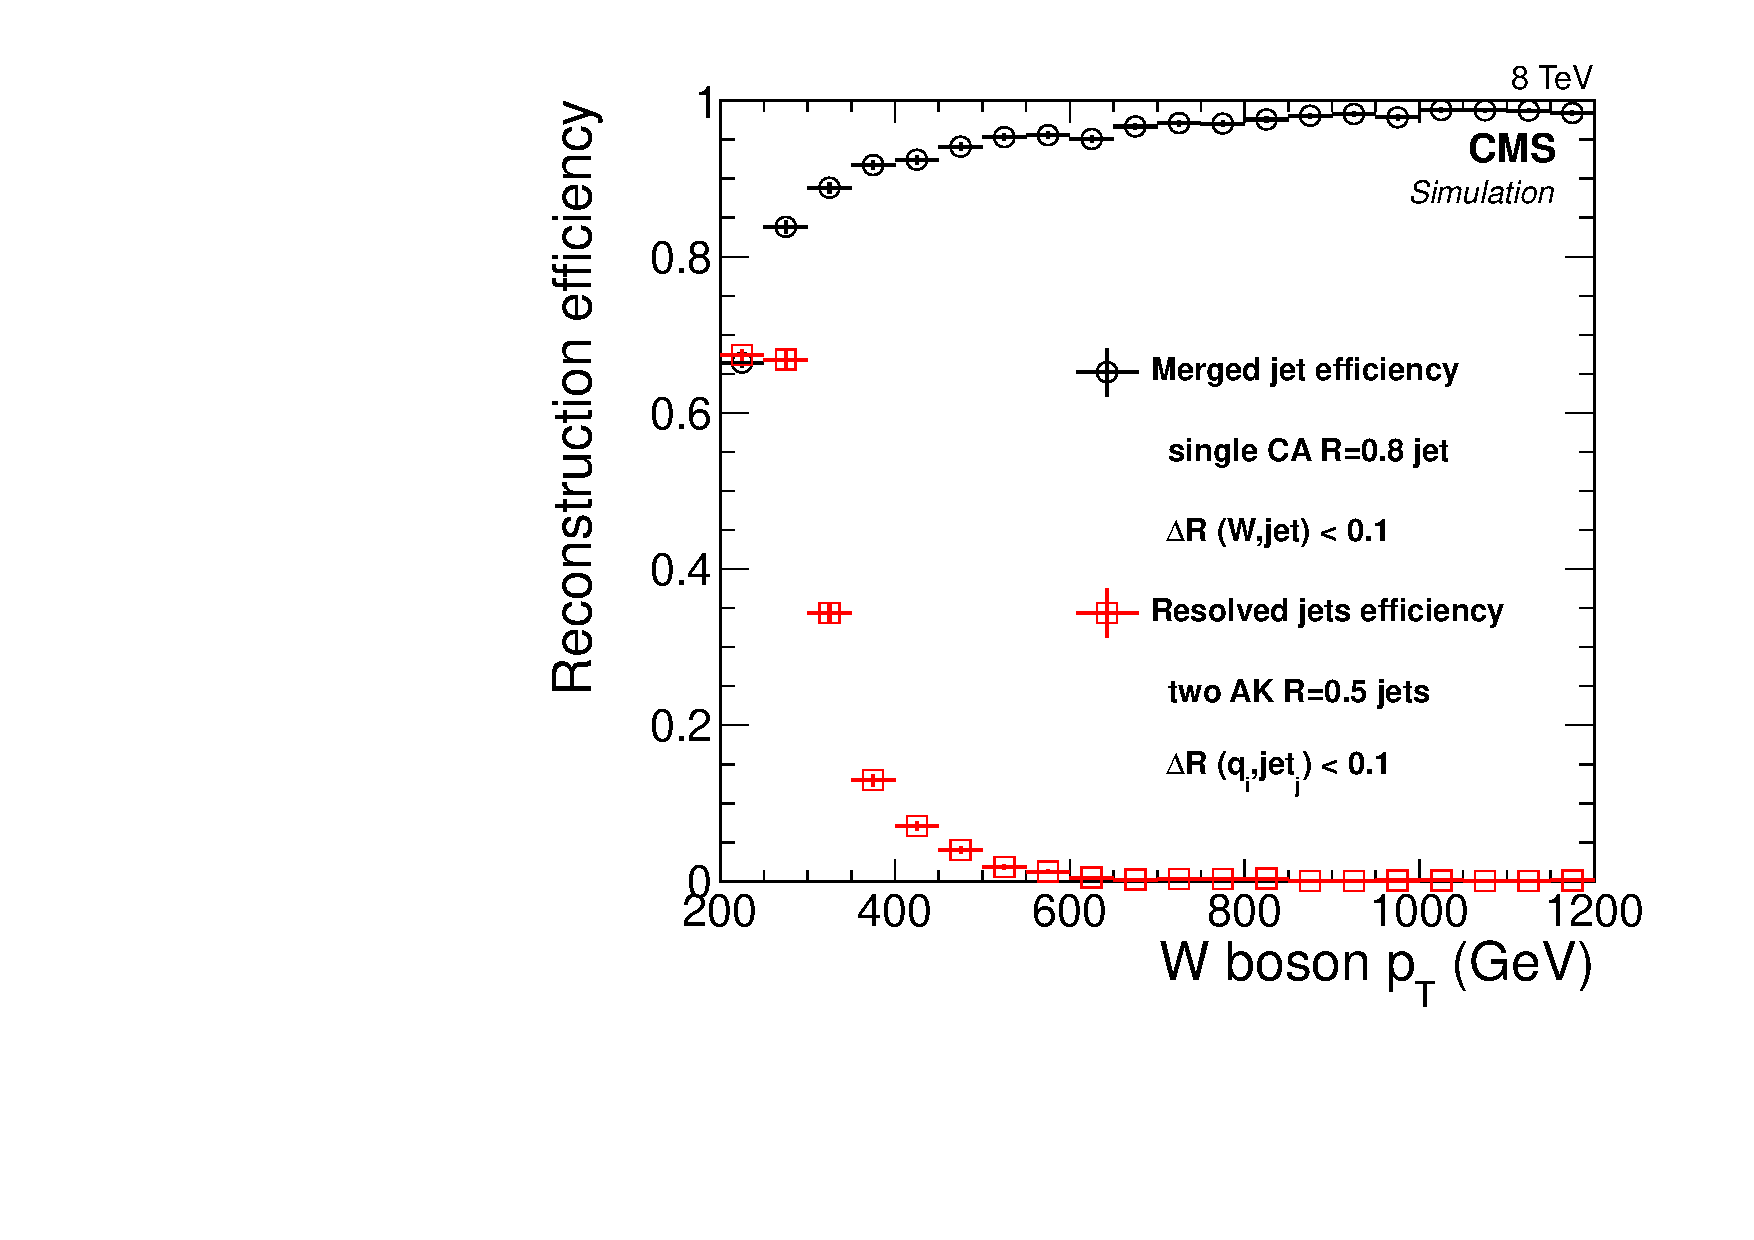
\includegraphics[width=0.45\textwidth]{\chsix/ca8effVsPt.pdf}
 \end{center}
 \caption{Efficiency to reconstruct a CA8 jet within $\Delta R <$ 0.1 of a generated W boson, and the efficiency to reconstruct two AK5 jets within $\Delta R <$ 0.1 of the generated quarks in the W-boson decay, as a function of the \pt of the W boson~\cite{Khachatryan:2014vla}.}
 \label{fig:ca8effVsPt}
\end{figure}

%%%%%%%% 
\subsection{Jet reconstruction and calibration}\label{subsec:jetsreco} %https://twiki.cern.ch/twiki/bin/view/CMSPublic/PhysicsResultsJME
%%%%%%%%

In CMS, the jet reconstruction is performed using the PF algorithm, which gives different reconstructed objects as input to the above-explained jet-clustering algorithms to build the so-called \textit{PF jets}.
%In CMS several standard methods for jet reconstruction are available which make use of different detector components, e.g. the tracker and the calorimeters, and give different reconstructed objects as input to the above explained jet clustering algorithms. In this work, only jets reconstructed with the PF algorithm are used and referred to as ``PF jets''.
%The so-called CaloJets are clustered from the energy measured in the electromagnetic and hadronic calorimeters (ECAL and HCAL) combined into towers. Jets can also be clustered from reconstructed charged particle tracks (TrackJets) or with the JetsPlusTracks (JPT) method [79] which combines reconstructed CaloJets with the information of the reconstructed tracks.
As sketched in Fig.~\ref{fig:PFalgo}, the PF algorithm aims at reconstructing all the stable particles produced in an event, combining the information coming from all CMS sub-detectors to optimize particle identification, direction and energy determination. These particles are classified in several types: charged hadrons, photons, neutral hadrons, electrons and muons. Jets are typically composed by 65\% charged hadrons, 25\% photons, 10\% neutral hadrons (Fig.~\ref{fig:PFjet_composition}). The PF algorithm is optimized to identify all these different components inside the jet, contrary to a calorimetric-only reconstruction. Typically, photons correspond to ECAL deposits not compatible with a tracker track. Charged hadrons correspond to HCAL and/or ECAL deposits matched to an inner track and not compatible with an electron, whereas neutral hadrons are identified as HCAL deposits not matched to any track.
%Particle trajectories measured in the tracker are extrapolated through the detector volume and are matched to the energy deposits in the calorimeters.
The momentum of neutral particles is obtained from the corresponding calorimeter energy deposits, calibrated for the non-linear response of the calorimeters.
For charged particles, the momentum is determined combining the track momentum measured by the tracker with high resolution and the corresponding calibrated calorimeter energy deposits.
%While the momentum of neutral particles is measured in the calorimeters, the momentum of charged particles is measured by the tracker with a better resolution.
Hence, both the position and energy measurements are greatly improved with respect to calorimeter jets as this algorithm makes use of the tracking detectors and high granularity of the ECAL which is much higher than that of the HCAL. Once all the PF candidates in the event are reconstructed, they are used as input to the jet-clustering algorithms described in the previous section and a PF jet is formed.
The jet momentum is determined as the vectorial sum of all PF candidates in the formed jet providing its ``raw'' estimate. 

\begin{figure}[!htb]
 \begin{center}
  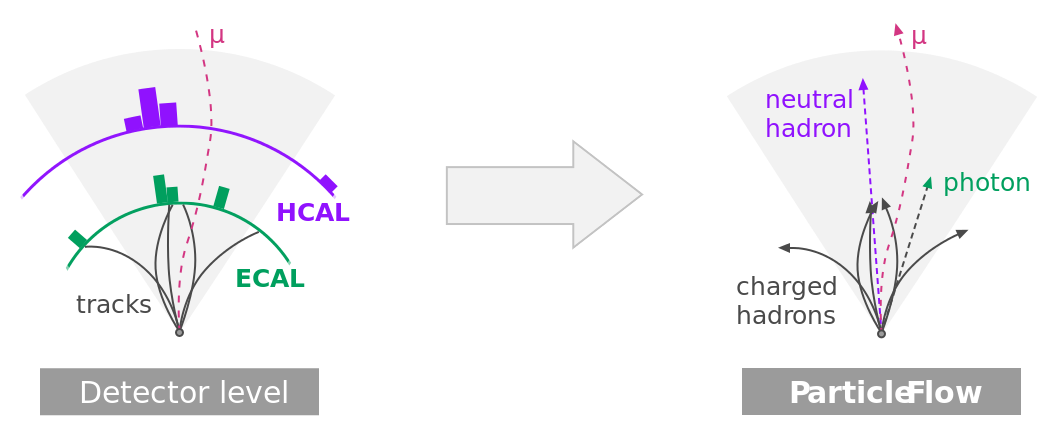
\includegraphics[width=0.7\textwidth]{\chsix/cms_particle_flow.png}
 \end{center}
 \caption{Sketch of the CMS particle-flow algorithm.}
 \label{fig:PFalgo}
\end{figure}

\begin{figure}[!htb]
\centering
\subfigure[]{\label{fig:PFjet_composition_a}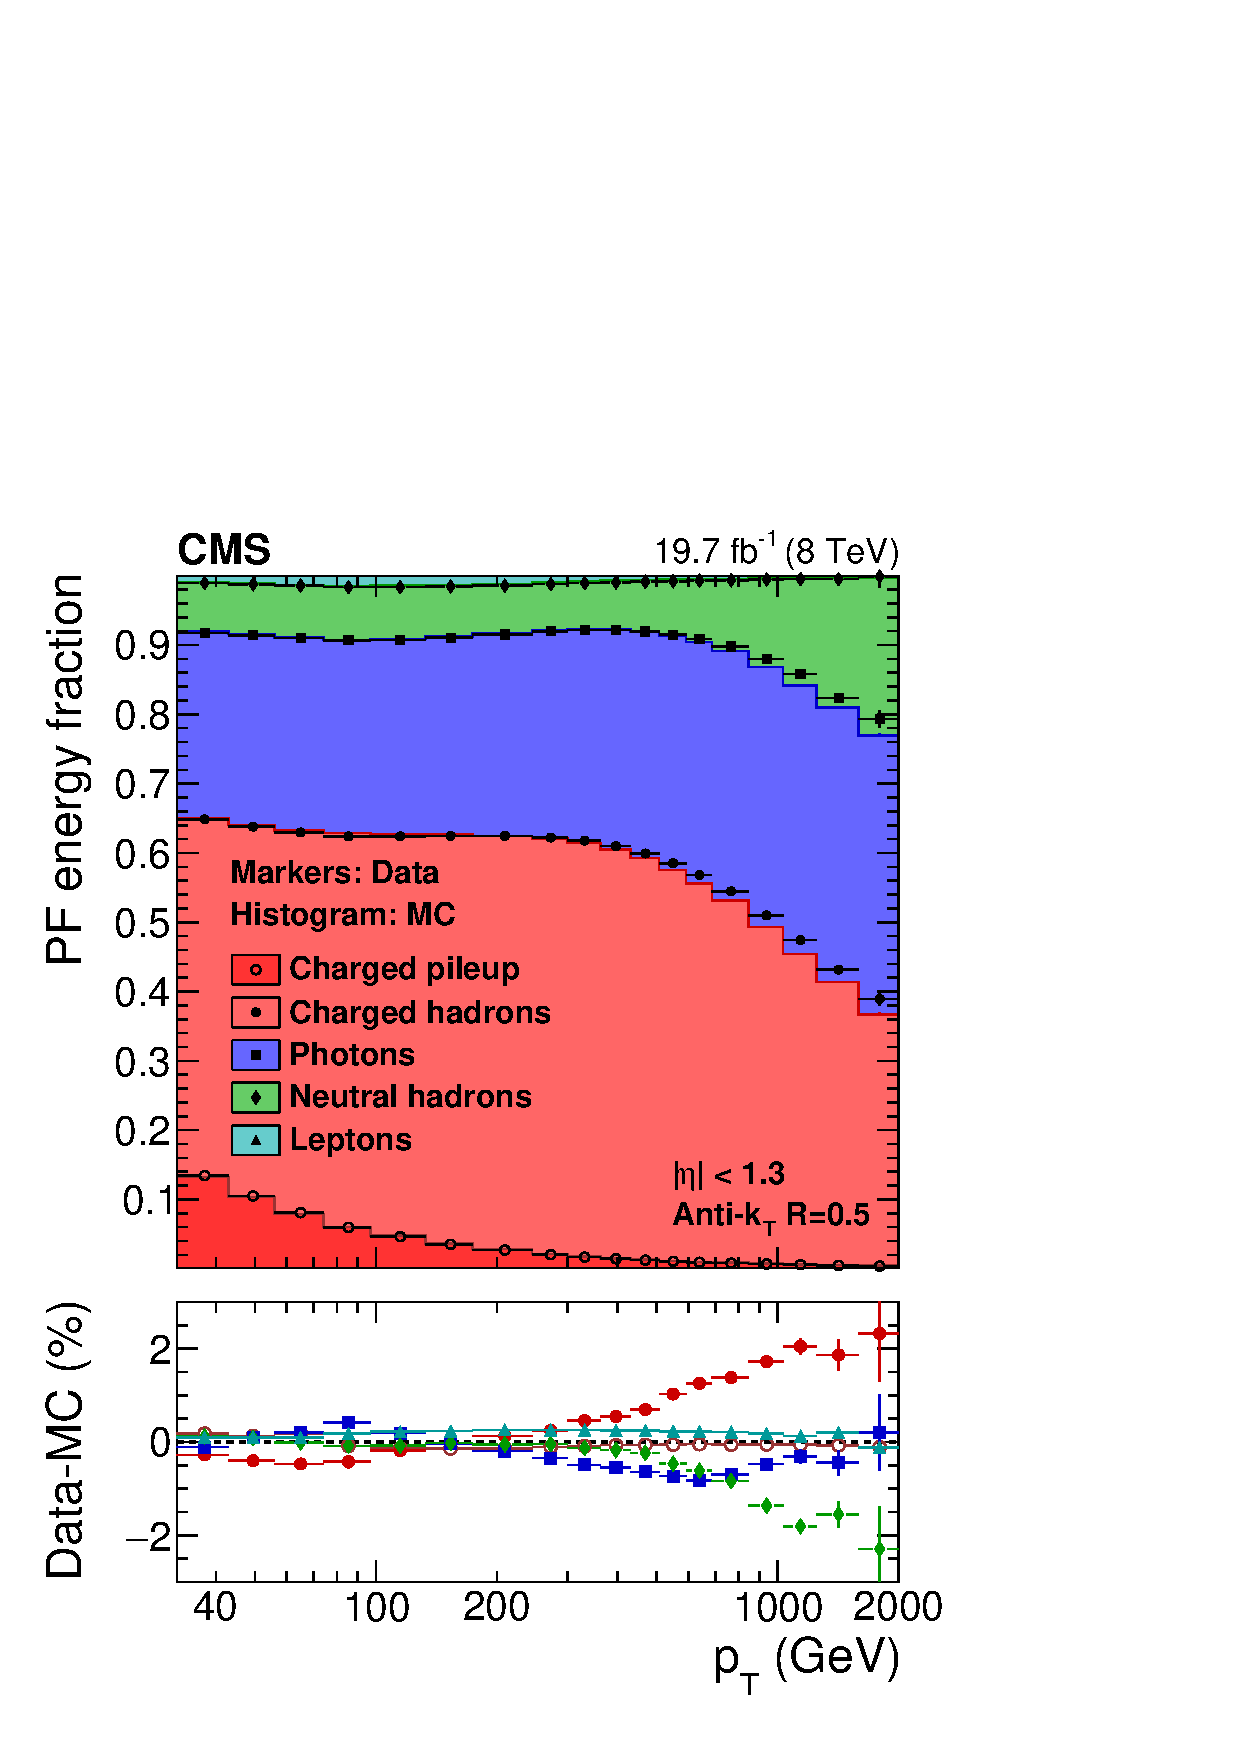
\includegraphics[width=0.45\textwidth]{\chsix/pfjet-composition-pt.pdf}}
\subfigure[]{\label{fig:PFjet_composition_b}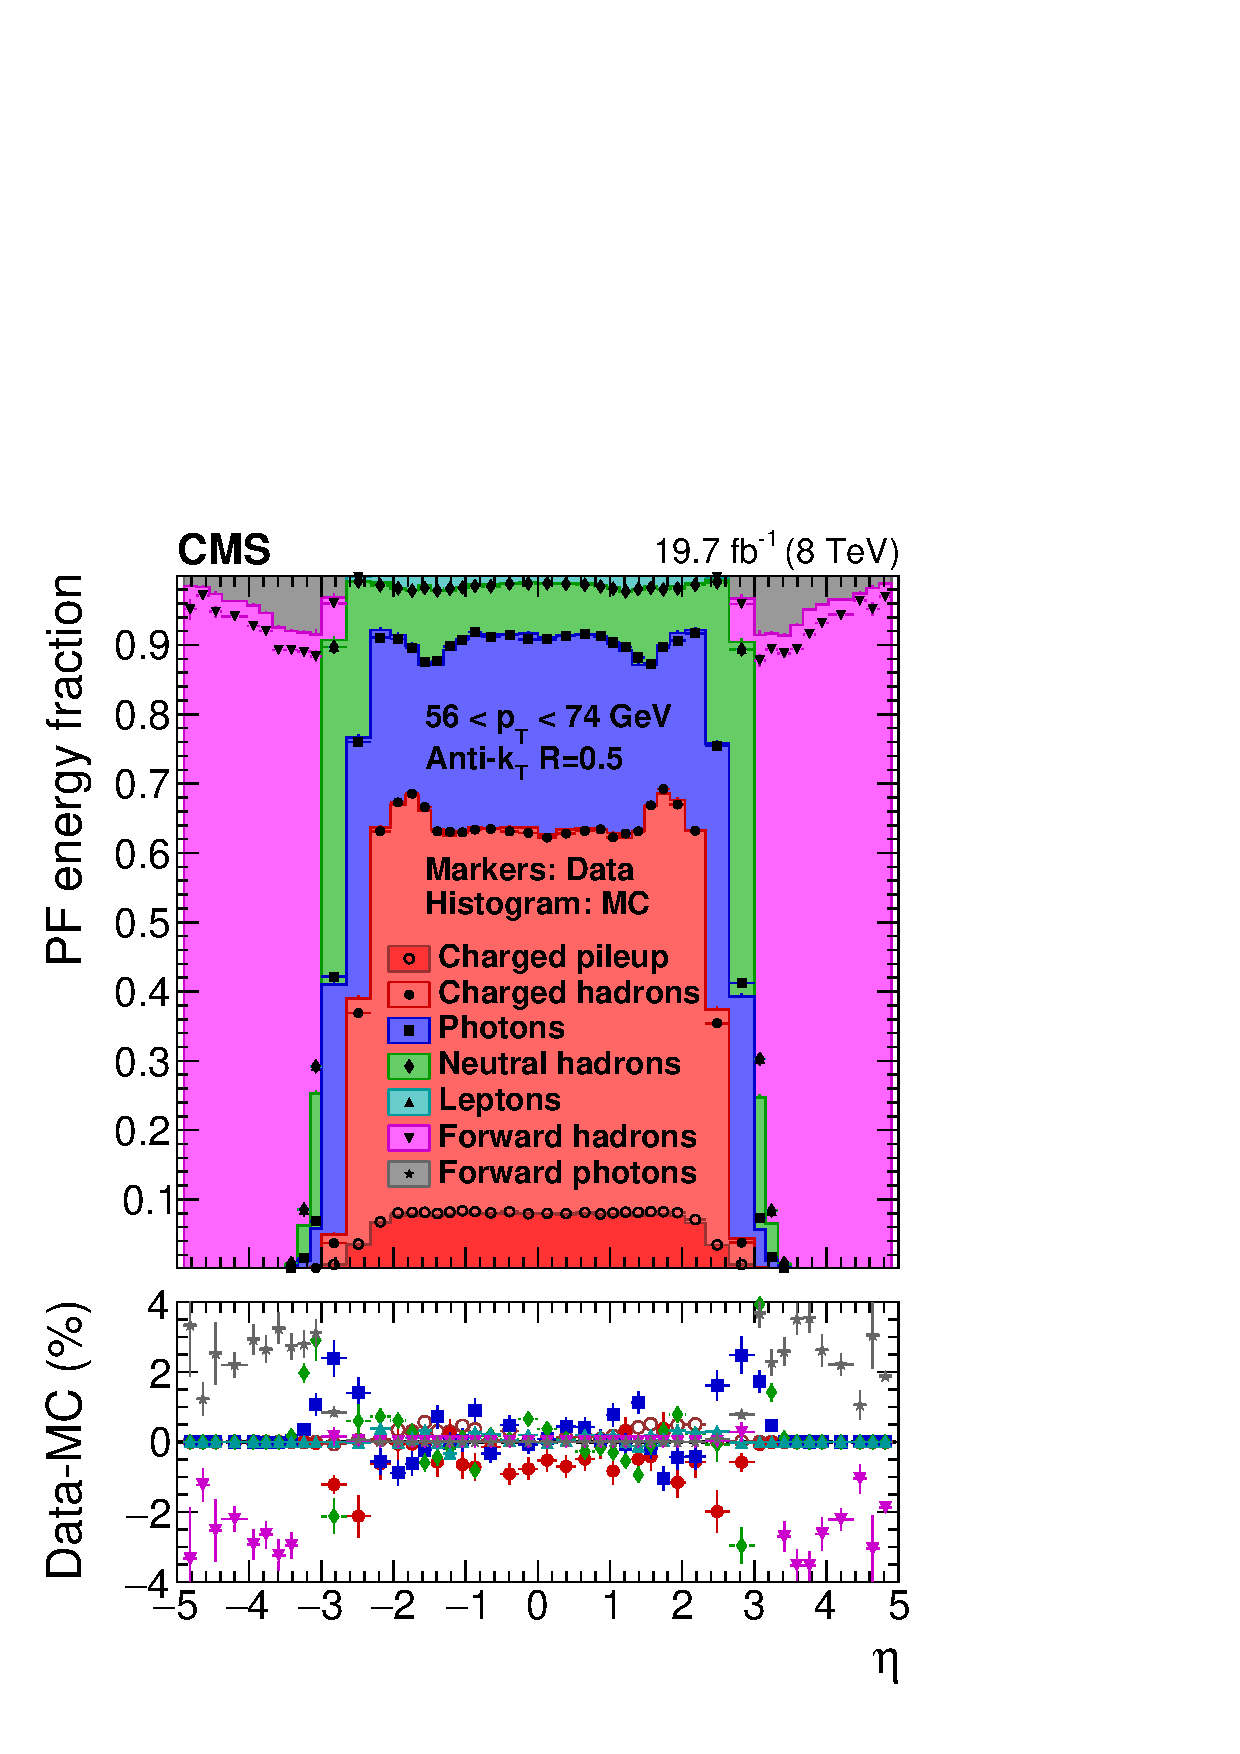
\includegraphics[width=0.45\textwidth]{\chsix/pfjet-composition-eta.pdf}}
\caption{PF jet composition in data and simulation as a function of jet \pt for jets with $|\eta| < 1.3$ (a), and as a function of $\eta$ for jets with \pt in the range $56 < \pt < 74\GeV$ (b)~\cite{Khachatryan:2016kdb}.}
\label{fig:PFjet_composition}
\end{figure}

The additional pp collisions occurring within the same bunch-crossing as the primary hard interaction produce additional tracks in the tracker and deposit energy in the calorimeters. This contribution is usually referred to as in-time pileup. Due to the finite signal decay time in the calorimeters, the pp collisions occurring in the previous and subsequent beam crossings also contribute to calorimetric energy in the same time window as the primary hard interaction. This contribution is called out-of-time pileup.
The out-of-time contribution is mitigated at the level of signal processing, while the in-time one is partially removed using tracking information. This is achieved by identifying which vertex the charged PF candidates originate from, and removing those unambiguously associated with pileup vertices before clustering jets. This method is referred to as \textit{charged-hadron subtraction} (CHS), and represents the reference standard method for jet reconstruction in CMS for Run~1 and beginning of Run~2.
%For the second part of Run~2, other pileup mitigation techniques in addition to CHS have been developed and tested in CMS~\cite{CMS-PAS-JME-13-005,CMS-PAS-JME-14-001,JME-16-003} but they are not used in this work. 

There are many possible sources of residual biases in the jet energy reconstruction, mainly due to the several intrinsic limitations of the system, such as the non-linear response of the calorimeters, the detector segmentation, the presence of material in front of calorimeters, electronic noise and pileup. The raw jet energy and resolution are thus corrected for several factors in order to obtain the energy value as close as possible to the true energy of the initial parton. CMS has adopted a factorized approach~\cite{1748-0221-6-11-P11002} to the problem of jet energy corrections, where each level of correction takes care of a different effect as described in the following.

The first step in this approach is a correction to the jet energies to mitigate additional pileup effects. 
In particular, the CHS jets are corrected to subtract residual contributions from neutral pileup particles, overlapping inside the jet cone. These corrections are determined from the simulation of a sample of QCD dijet events processed with and without pileup contaminations. This correction is usually parametrized as a function of the pileup energy density ($\rho$)~\cite{Cacciari:2011ma,Cacciari:2005hq}, the jet area (A)~\cite{Cacciari:2007fd}, jet \pt and $\eta$. The pileup offset corrections, defined as the mean value of the difference between the \pt of the reconstructed jet in events with and without pileup contamination, for AK5 CHS jets as a function of the corrected jet \pt and $\eta$ are shown in Fig.~\ref{fig:pucorr_ak5chs}, estimated for typical 2012 (8 TeV) conditions with an average number of additional pileup interactions $\left\langle\mu\right\rangle$ = 20.
The typical offset correction for a AK5 jet without CHS is 0.75 for a corrected jet \pt of 30\GeV, while a correction of 0.85 is obtained for AK5 CHS jets with same \pt value. This indicates that CHS removes approximately half of this offset before jet clustering by matching tracks to pileup vertices, reducing the residual offset correction. Roughly one third of the remaining pileup is from PF charged hadrons that have not been matched to good pileup vertices, and much of the rest is from PF photons. 

\begin{figure}[!htb]
\centering
\subfigure[]{\label{fig:pucorr_ak5chs_a}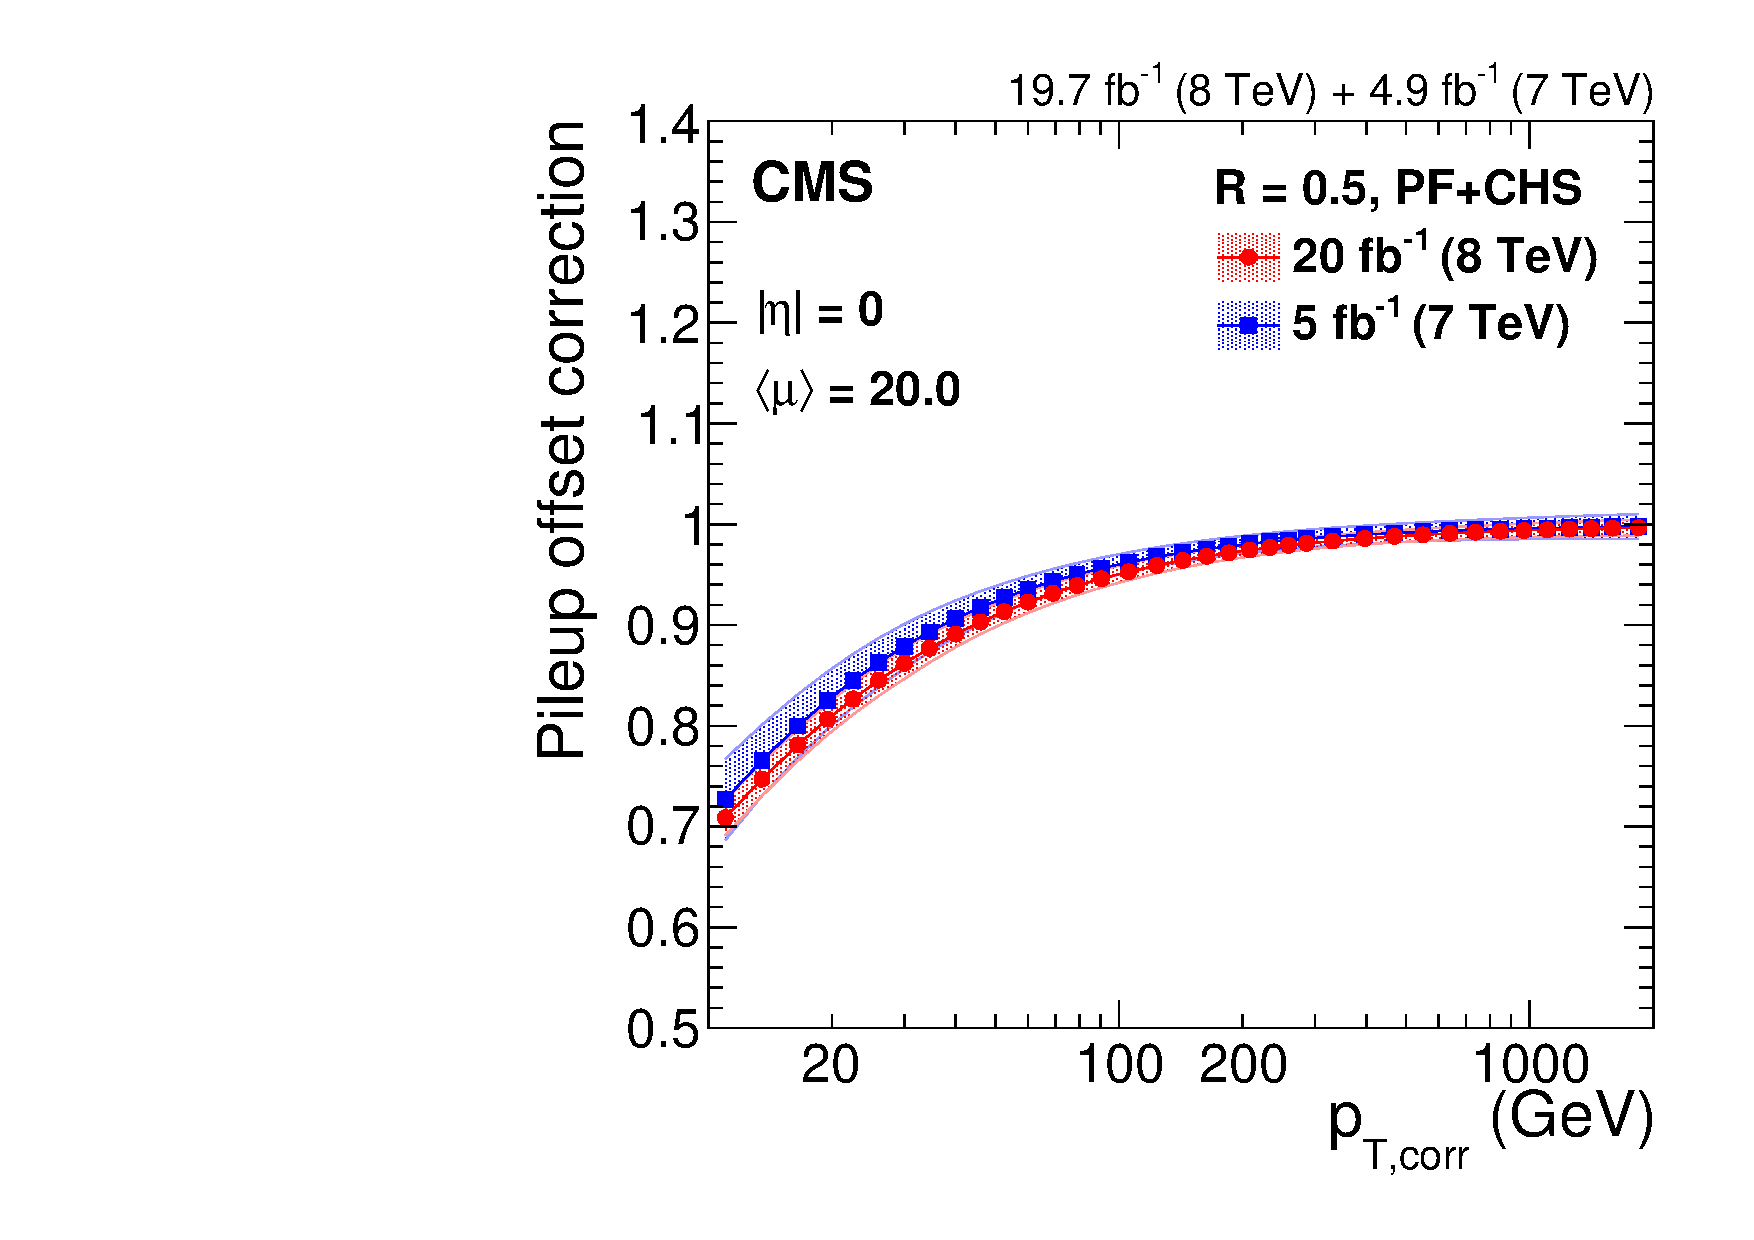
\includegraphics[width=0.45\textwidth]{\chsix/pu-corr-ak5chs-pt.pdf}}
\subfigure[]{\label{fig:pucorr_ak5chs_b}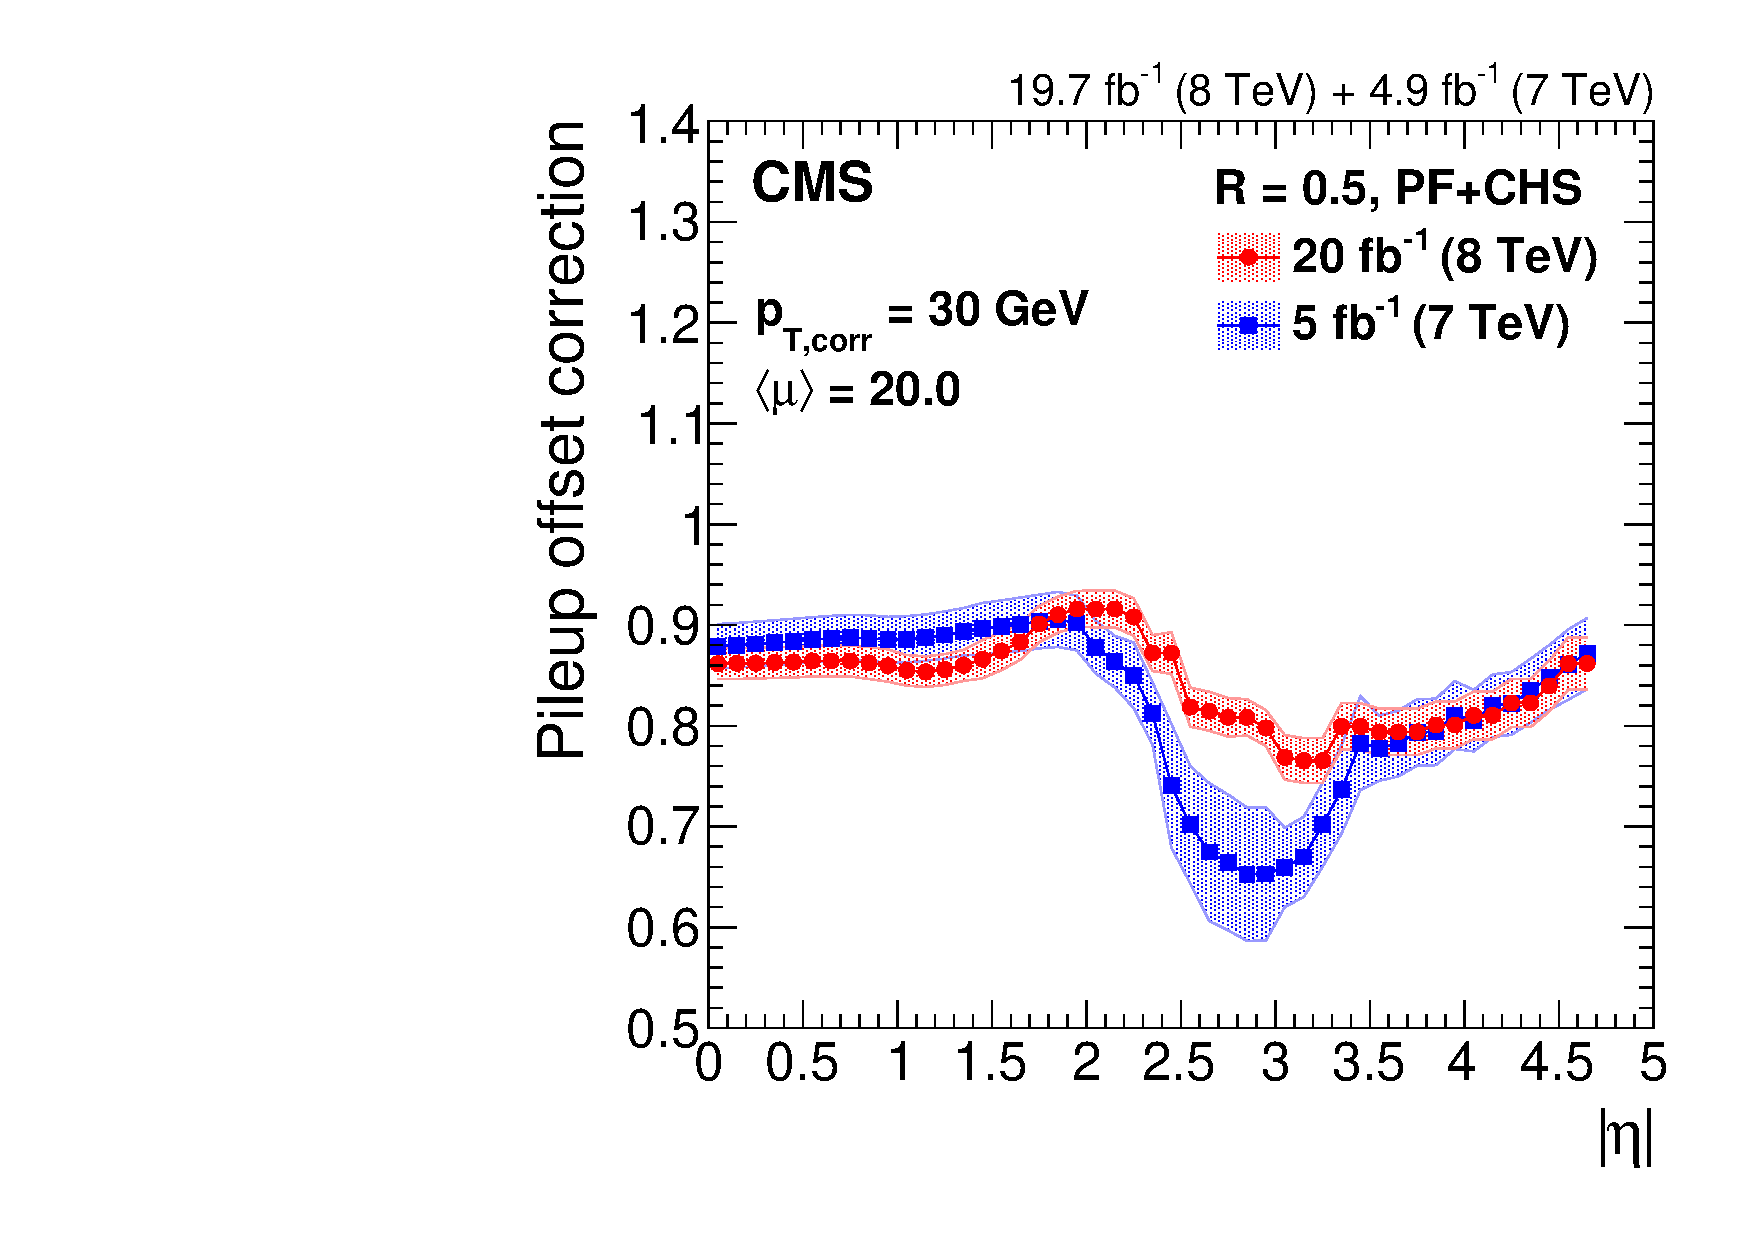
\includegraphics[width=0.45\textwidth]{\chsix/pu-corr-ak5chs-eta.pdf}}
\caption{Pileup offset correction for AK5 CHS jets estimated for the typical 2012 condition of $\left\langle\mu\right\rangle$ = 20. Corrections are shown for jets at $|\eta| = 0$ as a function of the corrected jet \pt (a), and for jets with $\pt = 30\GeV$ as a function of the jet $|\eta|$ (b)~\cite{Khachatryan:2016kdb}.}
\label{fig:pucorr_ak5chs}
\end{figure}

Secondly, a simulation-driven jet energy response correction is applied. The detector simulation takes into account effects due to
%particles deflected by the magnetic field,
energy lost when traversing the detector material, particle conversions, and a detailed detector geometry. In this step the aim is to correct for non-uniformities in the different CMS sub-detectors by comparing the reconstructed jet \pt to the particle-level one using simulated events only. The corrections are derived as a function of jet \pt and $\eta$ and make the response uniform over these two variables. The simulated particle response corrections are summarized in Fig.~\ref{fig:MCcorr_ak5chs} for 7 and 8\TeV data. The response is quite flat for $\pt > 50\GeV$, where the competing effects of increasing calorimeter response and falling tracking efficiency within the jet core compensate each other. In the barrel and endcap regions, the corrections rise with $|\eta|$, due to the increasing amount of material located in front of the calorimeters, which leads to effects such as an increased rate of nuclear interactions in the tracker. The corrections are higher around $|\eta|$ = 1.3 and 3.0 due to the degradation of the response in the transition regions.

\begin{figure}[!htb]
\centering
\subfigure[]{\label{fig:MCcorr_ak5chs_a}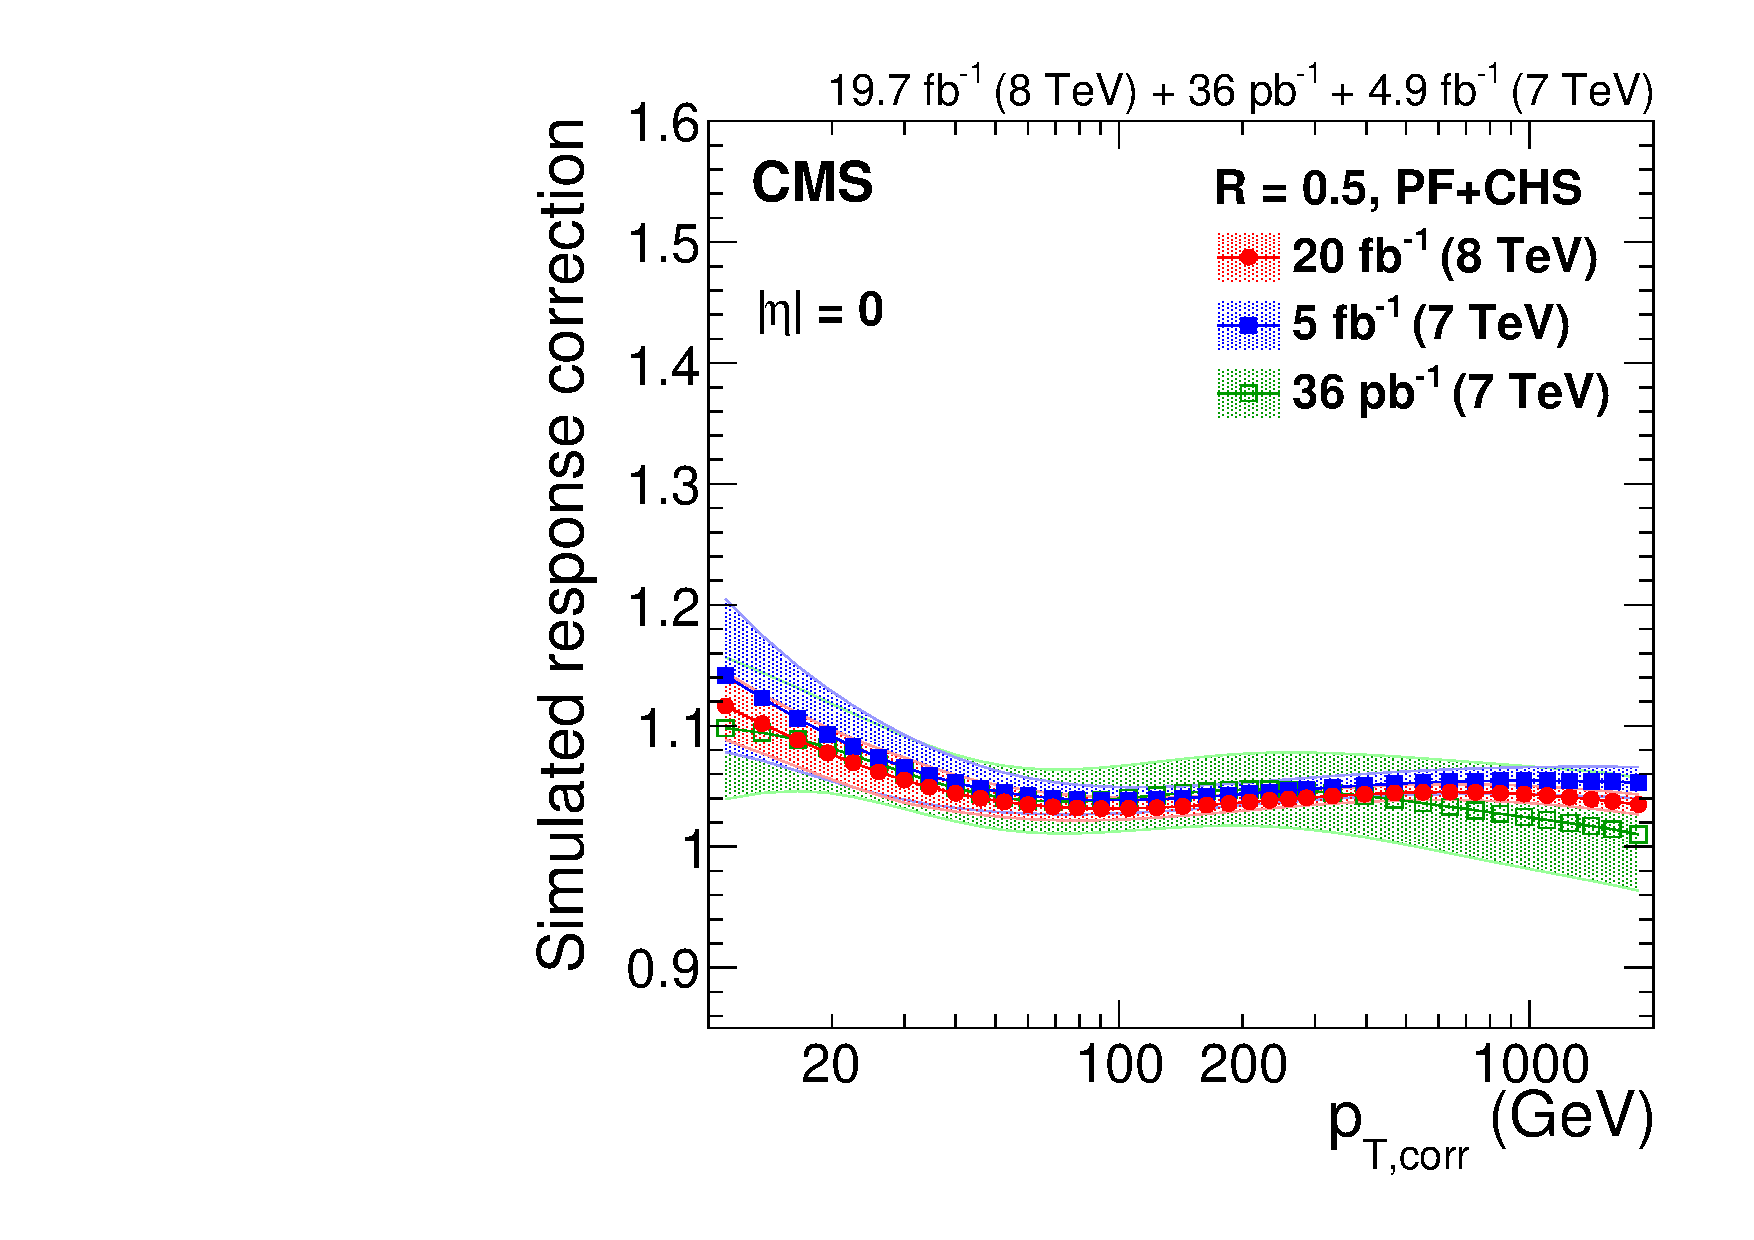
\includegraphics[width=0.45\textwidth]{\chsix/mc-corr-ak5chs-pt.pdf}}
\subfigure[]{\label{fig:MCcorr_ak5chs_b}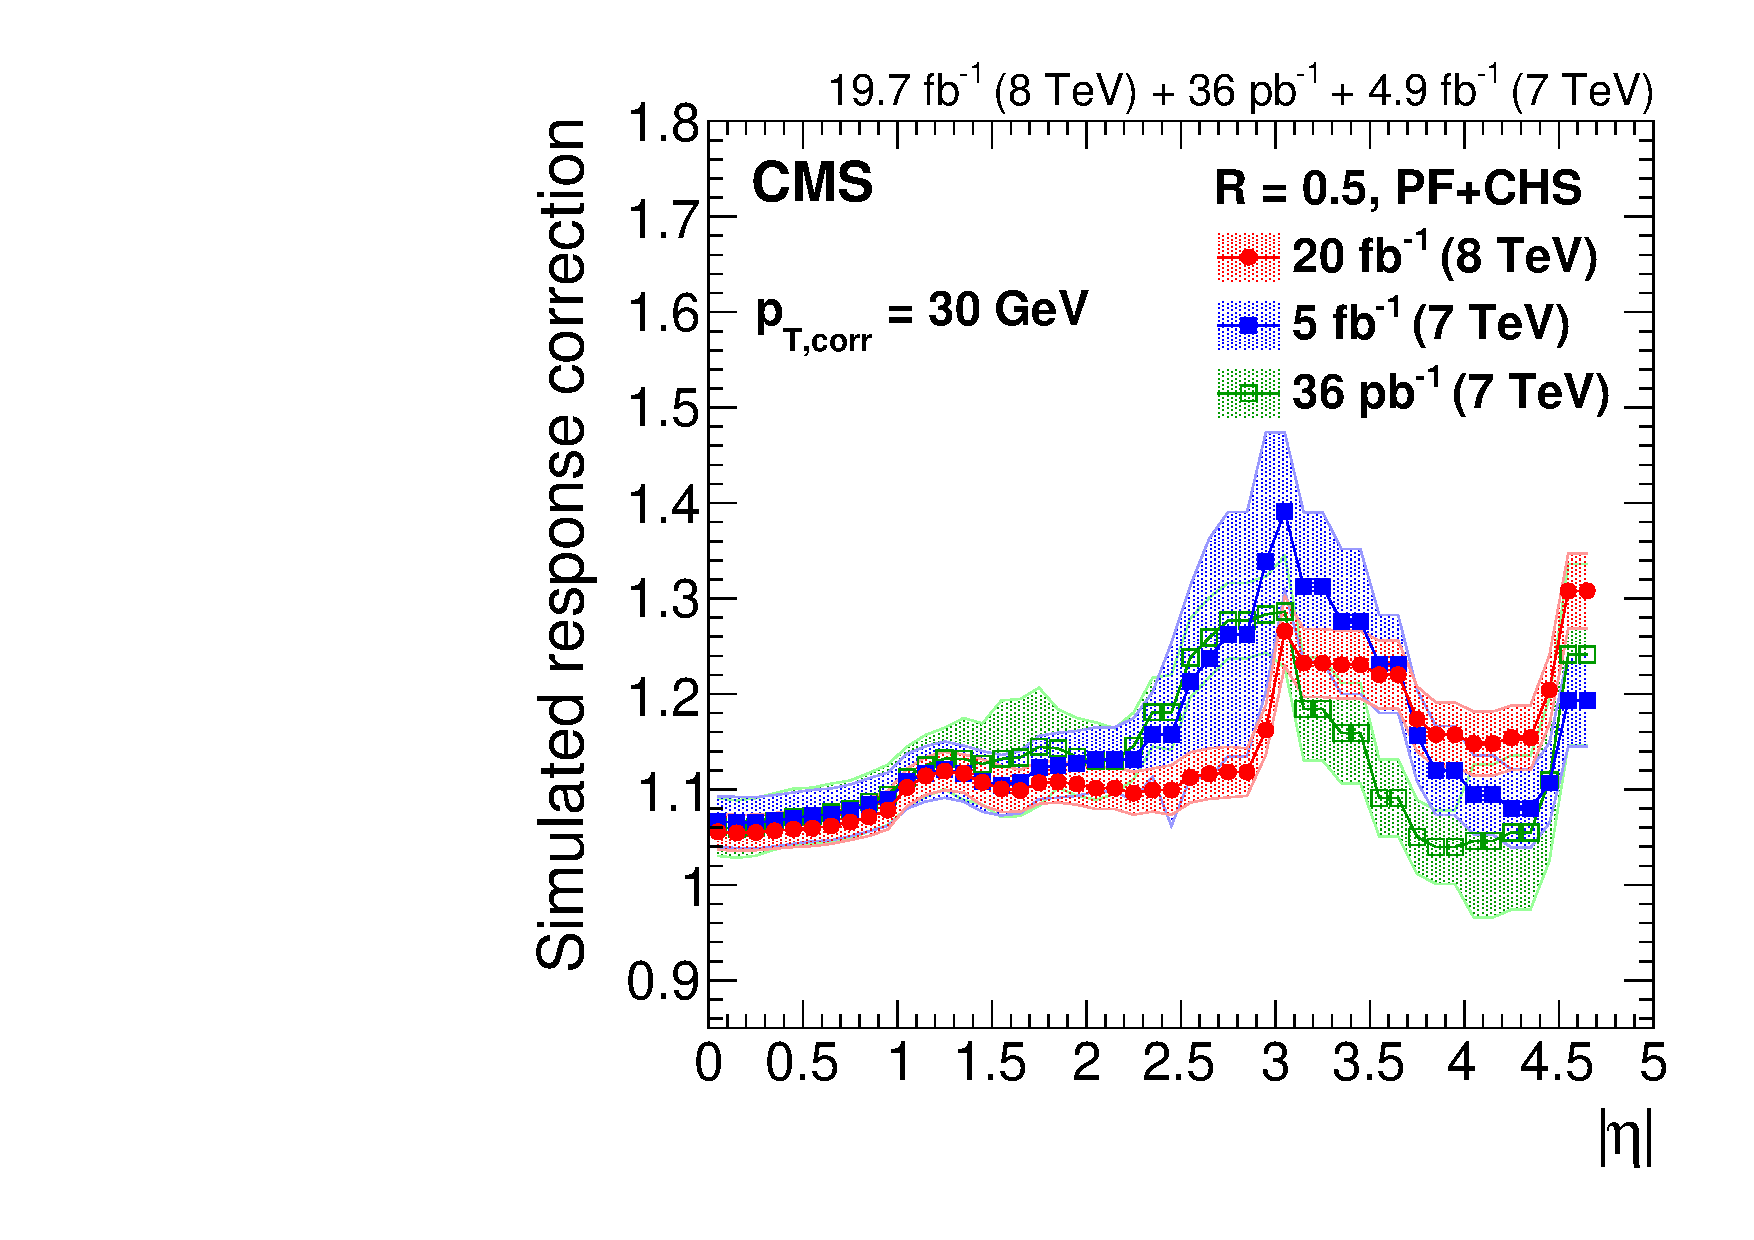
\includegraphics[width=0.45\textwidth]{\chsix/mc-corr-ak5chs-eta.pdf}}
\caption{Detector response correction factors for AK5 CHS jets estimated for the 8\TeV data collected in 2012. Corrections are shown for jets at $|\eta| = 0$ as a function of the corrected jet \pt (a), and for jets with $\pt = 30\GeV$ as a function of the jet $|\eta|$ (b)~\cite{Khachatryan:2016kdb}.}
\label{fig:MCcorr_ak5chs}
\end{figure}

Finally data-driven residual corrections are applied to correct for any measurable difference between the detector simulation and the jets measured in data. 
%This correction is done in two steps: first, the calibration as a function of jet $\eta$, and second, as a function of $\pt$.
This correction is done in two steps. At first, an additional correction for the non-homogeneous response of the detector with $\eta$ is derived from dijet events, in which the \pt response of a probe jet, outside the barrel region, is balanced with the one in the reference tag region ($|\eta| < 1.3$) as a function of the average \pt of the dijet system. Only events with back-to-back dijets and little additional activity in the event are used to avoid any impact from unbalanced events. %The result of the \pt-dependent fit is shown in Fig.~\ref{fig:rescorr_ak5chs_a}.
The jet energy is calibrated as a function of transverse momentum using a combination of Z($\to\ell\ell$)+jet, $\gamma$+jet, and multijet events for jets in the reference barrel region ($|\eta| < 1.3$). The basic idea, in all the considered topologies, is to exploit the transverse momentum balance between the jet to be calibrated and a well-reconstructed and calibrated reference object (Z or $\gamma$). The jet energy response is studied using two approaches. In one method the jet response is evaluated by comparing the reconstructed jet momentum ($p_\mathrm{T,jet}$) directly to the momentum of the reference object ($p_\mathrm{T,ref}$), while the second, more advanced, method takes into account the missing energy measured in the calorimeters to balance the reference object and jet momenta. In this method the additional event activity is taken into account by the missing energy. Therefore, additional jets in the event have only a small impact on the measurement. The residual corrections are summarized in Fig.~\ref{fig:rescorr_ak5chs} for 8\TeV data. The residual response corrections are less than 3\% in the barrel, less than 10\% in the endcaps, and about 10\% in the forward detector.

\begin{figure}[!htb]
\centering
\subfigure[]{\label{fig:rescorr_ak5chs_a}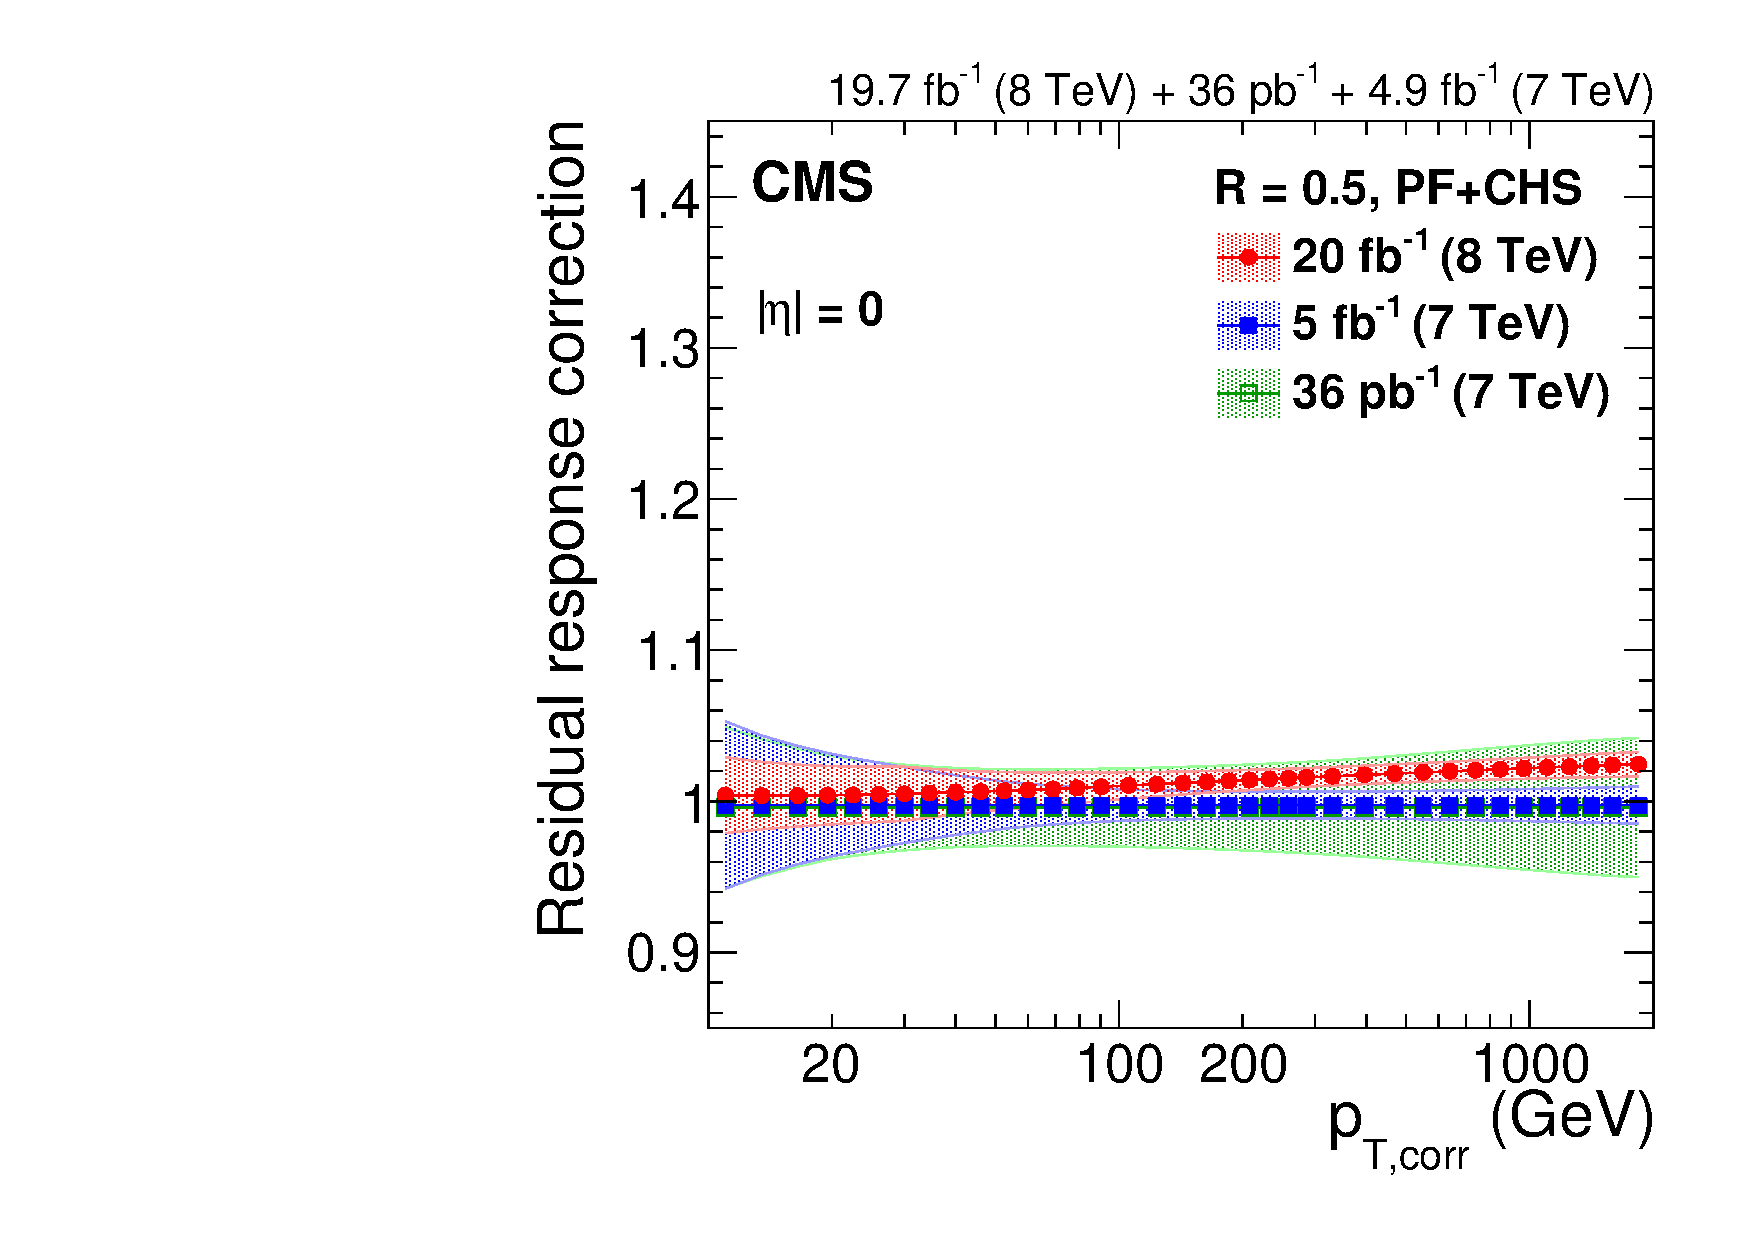
\includegraphics[width=0.45\textwidth]{\chsix/res-corr-ak5chs-pt.pdf}}
\subfigure[]{\label{fig:rescorr_ak5chs_b}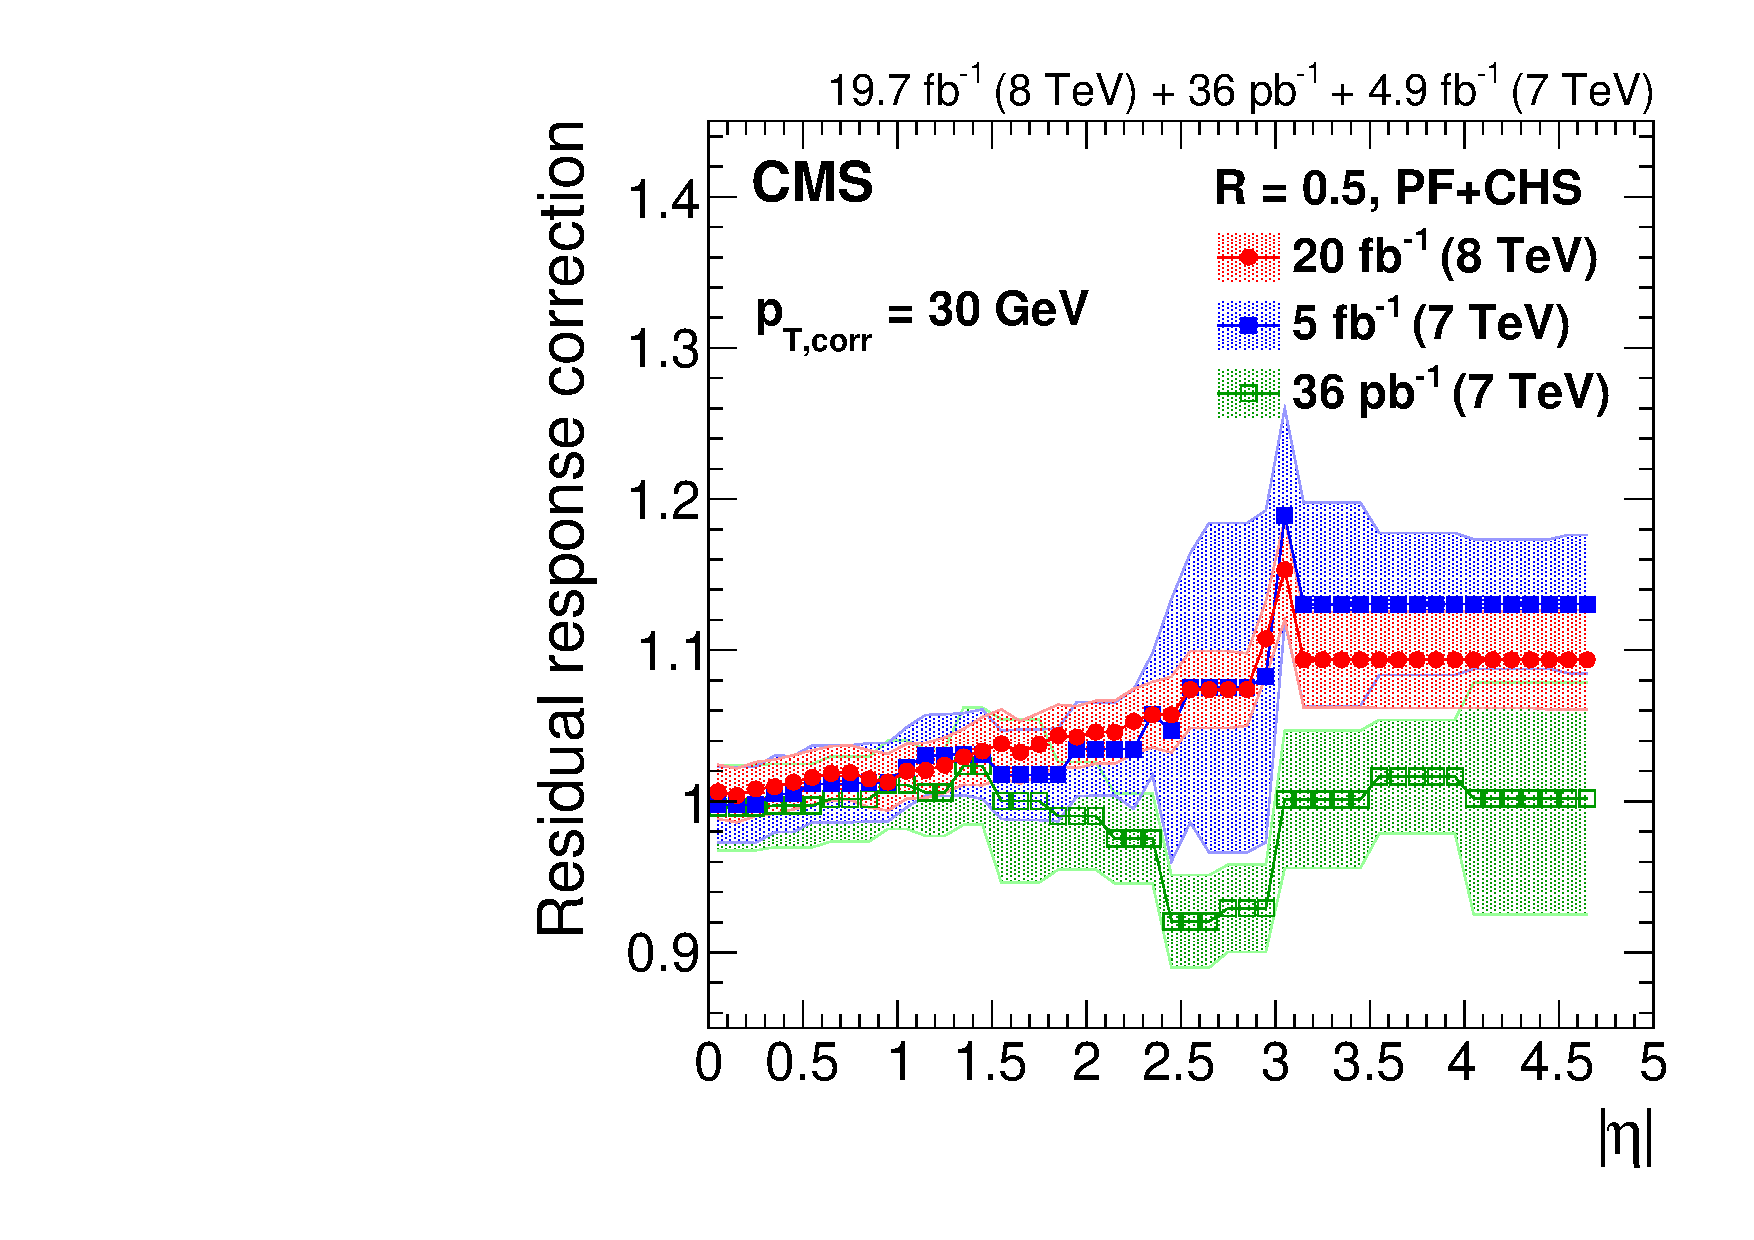
\includegraphics[width=0.45\textwidth]{\chsix/res-corr-ak5chs-eta.pdf}}
\caption{Residual data/simulation response correction factors for AK5 CHS jets for the 8\TeV data collected in 2012. Corrections are shown for jets at $|\eta| = 0$ as a function of the corrected jet \pt (a), and for jets with $\pt = 30\GeV$ as a function of the jet $|\eta|$ (b)~\cite{Khachatryan:2016kdb}.}
\label{fig:rescorr_ak5chs}
\end{figure}

The fully-calibrated PF jets are finally obtained in both data and simulation by multiplying all the above correction factors to the raw jet \pt as follows:

\begin{equation}
p_\mathrm{T,corr} = p_\mathrm{T,raw} \times C_\mathrm{pu}(p_\mathrm{T,raw},\eta,\rho\cdot\mathrm{A}) \times C_\mathrm{sim}(C_\mathrm{pu} \cdot p_\mathrm{T,raw},\eta) \times C_\mathrm{res}(C_\mathrm{pu} \cdot C_\mathrm{sim} \cdot p_\mathrm{T,raw},\eta)
\end{equation}

where $C_\mathrm{pu}$ represents the pileup correction, $C_\mathrm{sim}$ is the simulated response correction and $C_\mathrm{res}$ is the global residual correction applied only on jets in data.
Figure~\ref{fig:jesunc813TeV} shows the overall uncertainty on the corrections to the jet energy scale for AK5 and AK4 CHS jets for 8 and 13\TeV data, respectively. In both cases, the final uncertainties are below 3\% across the phase space of this analysis.

\begin{figure}[!htb]
\centering
\subfigure[]{\label{fig:jesunc_ak5chs_a}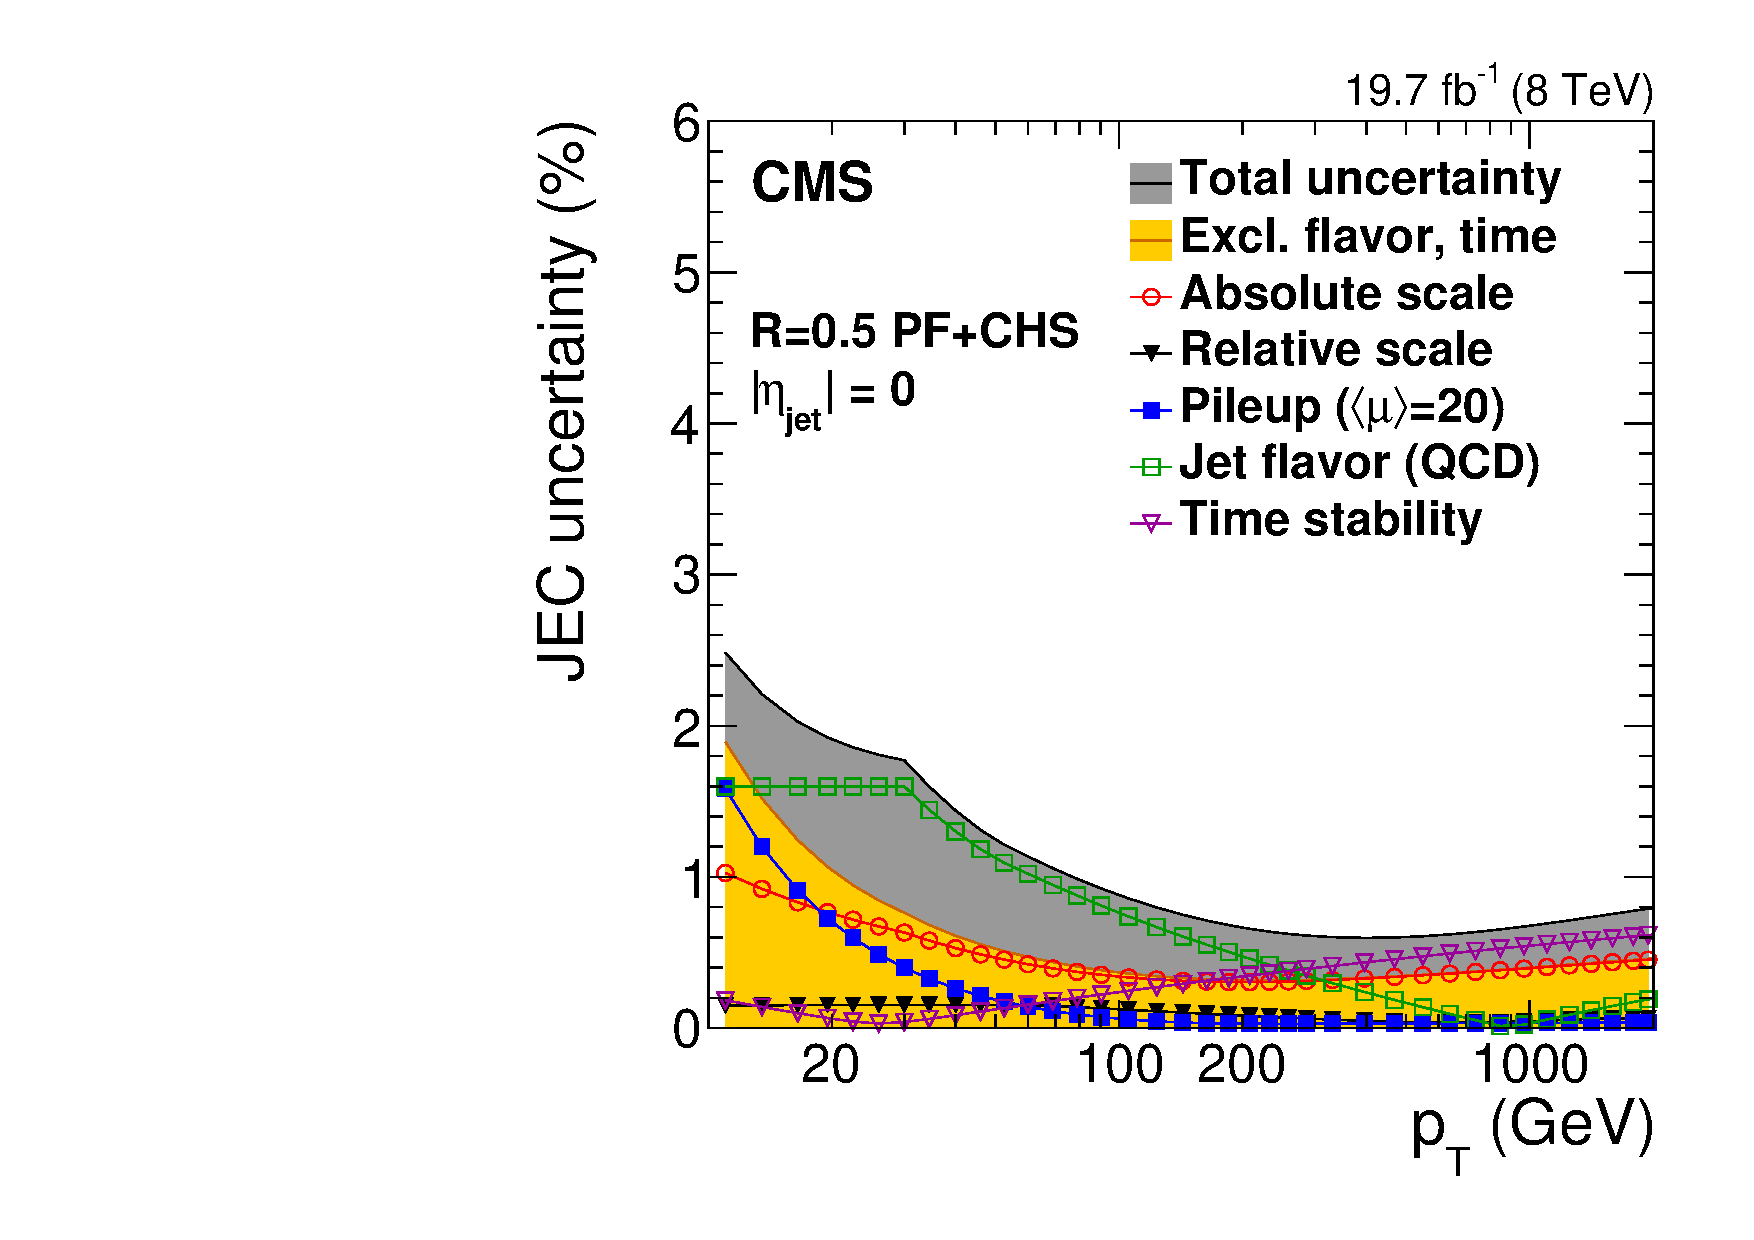
\includegraphics[width=0.45\textwidth]{\chsix/jesunc-ak5chs-pt.pdf}}
\subfigure[]{\label{fig:jesunc_ak5chs_b}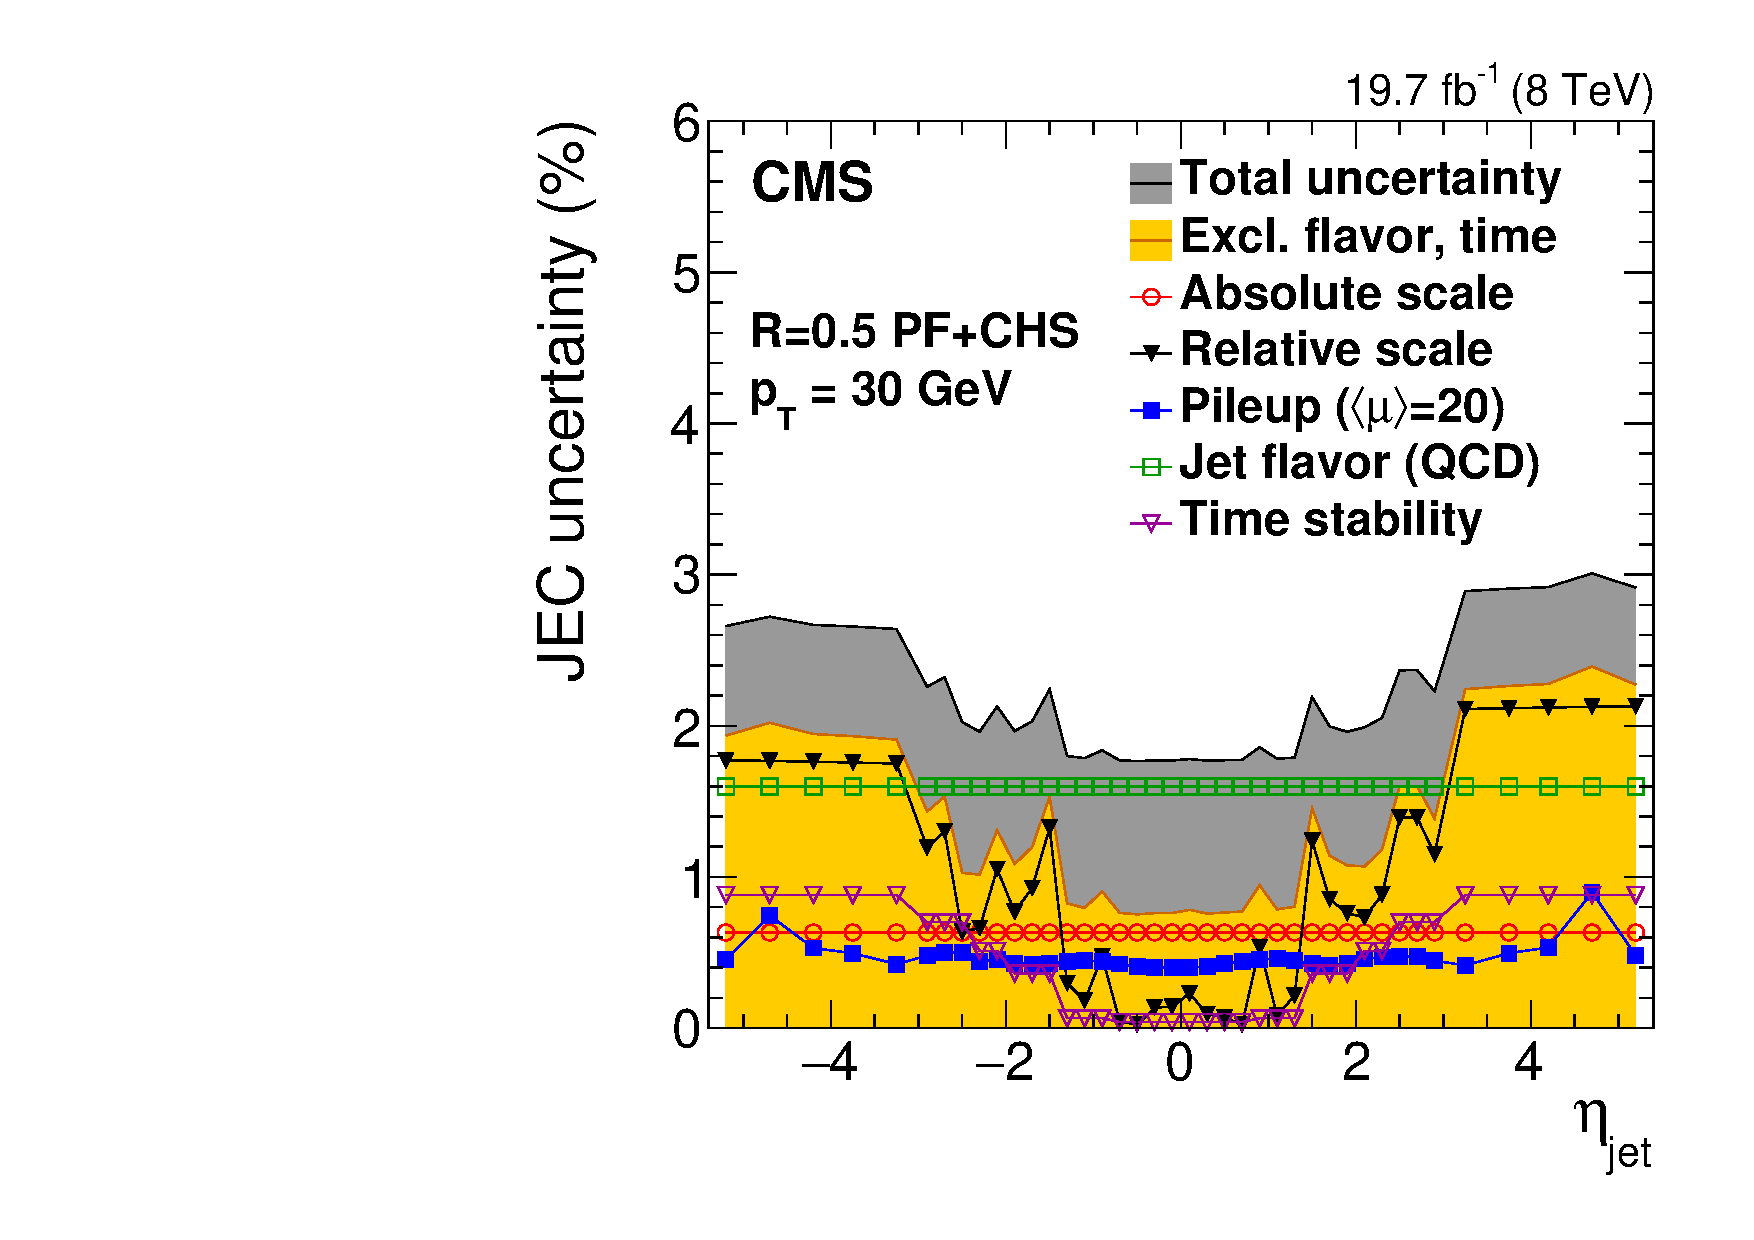
\includegraphics[width=0.45\textwidth]{\chsix/jesunc-ak5chs-eta.pdf}}\\
\subfigure[]{\label{fig:jesunc_ak4chs_c}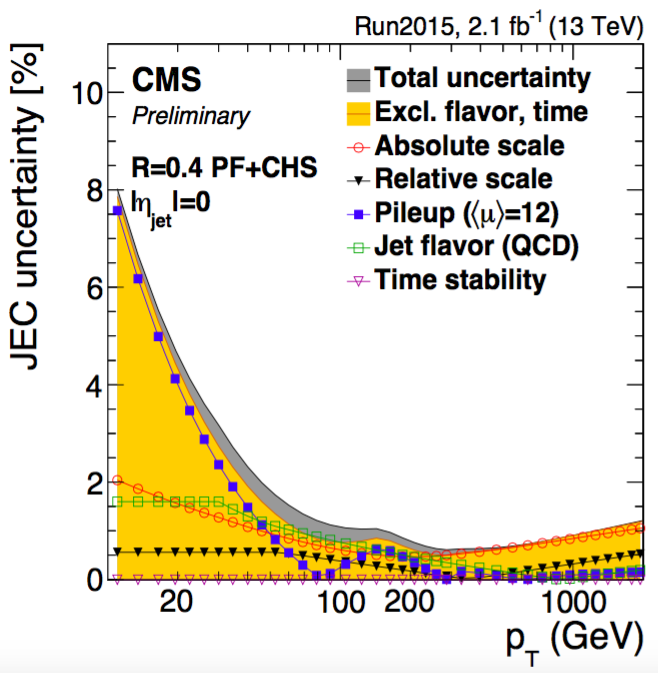
\includegraphics[width=0.45\textwidth]{\chsix/jesunc-ak4chs-pt.png}}
\subfigure[]{\label{fig:jesunc_ak4chs_d}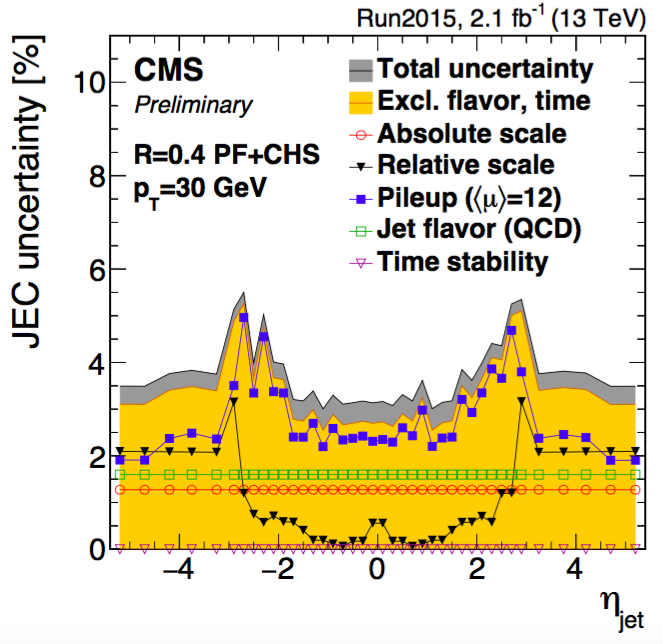
\includegraphics[width=0.45\textwidth]{\chsix/jesunc-ak4chs-eta.png}}
\caption{Summary of jet energy scale systematic uncertainties for the 8\TeV data collected in 2012 for AK5 CHS jets (upper plots) and for the 13\TeV data collected in 2015 for AK4 CHS jets (lower plots). Uncertainties are shown for jets at $|\eta| = 0$ as a function of the corrected jet \pt (left), and for jets with $\pt = 30\GeV$ as a function of the jet $|\eta|$ (right)~\cite{Khachatryan:2016kdb,CMS-DP-2016-020}.}
\label{fig:jesunc813TeV}
\end{figure}

The energy resolution of jets is relatively poor compared to the resolution of other physics objects (electrons, muons, photons), and the biases caused by jet resolution smearing are important for steeply falling spectra and for resonance decays. Hence, calibrations are evaluated to correct the jet energy resolution in addition to the corrections to the jet energy scale described above. The measurements are performed with methods which are extensions of the methods used for measuring jet energy scales, but instead of looking at the mean of the response distribution, the width is the interesting parameter. Furthermore, corrections have to compensate for effects that do not produce an overall shift in the mean, but that can widen the distribution. As shown in Fig.~\ref{fig:resolcorr813TeV}, the jet energy resolution in data is worse than in the simulation by 10--20\% depending on $\eta$, and the jets in simulation need to be smeared accordingly.\\
%Typical jet energy resolutions at the central rapidities are 15--20\% at 30\GeV, about 10\% at 100\GeV, and 5\% at 1\TeV. 
%The total uncertainty varies between 3--8\% for $|\eta| < 2.3$, increasing toward higher rapidity.

Jets used in this analysis are requested to pass loose identification criteria, in order to reject spurious jet-like features originating from isolated noise patterns in the calorimeters or the tracker. The efficiency of these requirements is above 99\% for real jets~\cite{CMS-PAS-JME-10-003}. 

For the 8\TeV data analysis described in this work, all AK5 and CA8 jets must have corrected $\pt > 30\GeV$ and $> 200\GeV$, respectively, and $|\eta| < 2.4$ to be considered in the subsequent steps of the analysis.
Furthermore, the AK5 and CA8 jets are required to be separated from any well-identified muon or electron (Sections~\ref{sec:muons} and~\ref{sec:electrons}) by $\Delta R > 0.3$ and $> 0.8$, respectively. This requirement is applied to clean the jet collection used in the analysis from leptons clustered in jets. The AK5 jets are required to be separated from the CA8 jet representing the $\PV\to\qqbar$ candidate by $\Delta R > 0.8$ since an overlap is expected between the two reconstructions. Finally, CA8 jets are not used in the analysis if their pseudorapidity falls in the region $1.0 < |\eta| < 1.8$, thus overlapping the barrel-endcap transition region of the silicon tracker.
In fact, in Run~1 it has been found that in this region, `noise' can arise when the tracking algorithm reconstructs many fake displaced tracks associated with the jet.
This issue in the reconstruction has been studied in detail in the context of this work. The studies, presented and discussed in Appendix~\ref{app:tobtec}, resulted in the choice of the $\eta$ region to be excluded.
In particular, the simulation does not sufficiently describe the full material budget of the tracking detector in that region, thus it does not accurately describe this effect.
Without this requirement, a bias can be introduced in the b-tagging, jet-substructure and missing energy information, making this analysis systematically prone to that noise.
As a consequence of these results, other analyses involving similar kinematic cuts and identification algorithms have been affected~\cite{CMS-PAS-EXO-15-008}.
The same selections are applied for AK4 and AK8 jets in the 13\TeV data analysis, except for the fiducial cut on the $\eta$ of the large-cone jet since the aforementioned reconstruction issue has been fixed for Run~2.
%For the 13\TeV data analysis described in this work, all AK4 and AK8 jets must have corrected $\pt > 30\GeV$ and $> 200\GeV$, respectively, and $|\eta| < 2.4$ to be considered in the subsequent steps of the analysis.
%Furthermore, the AK4 and AK8 jets are required to be separated from any well-identified muon or electron (Sections~\ref{sec:muons} and~\ref{sec:electrons}) by $\Delta R > 0.3$ and $> 0.8$, respectively. This requirement is applied to clean the jet collection used in the analysis from leptons misidentified as jets. Finally, AK4 jets are required to be separated from the AK8 jet representing the $\PV\to\qqbarpr$ candidate by $\Delta R > 0.8$ since an overlap is expected between the two reconstructions. The same selections are applied for AK5 and CA8 jets in the 8\TeV data analysis. For this case an additional selection is applied to the pseudorapidity of CA8 jets.
%In particular, CA8 jets are not used in the analysis if their pseudorapidity falls in the region $1.0 < |\eta| < 1.8$, thus overlapping the barrel-endcap transition region of the silicon tracker.
%In fact, in Run~1 it has been found that in this region, `noise' can arise when the tracking algorithm reconstructs many fake displaced tracks associated with the jet.
%This issue in the reconstruction has been studied in details in the context of this work. The studies, presented and discussed in Appendix~\ref{app:tobtec}, resulted in the choice of the $\eta$ region to be excluded.
%In particular, the simulation does not sufficiently describe the full material budget of the tracking detector in that region, thus it does not accurately describe this effect.
%Without this requirement, a bias can be introduced in the b tagging, jet substructure and missing energy information, making this analysis systematically prone to that noise.
%As a consequence of these results, other analyses involving similar kinematic cuts and identification algorithms have been affected~\cite{CMS-PAS-EXO-15-008}.
%However, this problem has been fixed for Run~2 and this additional fiducial cut does not have to be applied in 13\TeV data analyses.

\begin{figure}[!htb]
\begin{center}
%\subfigure[]{\label{fig:resolcorr_ak5chs_a}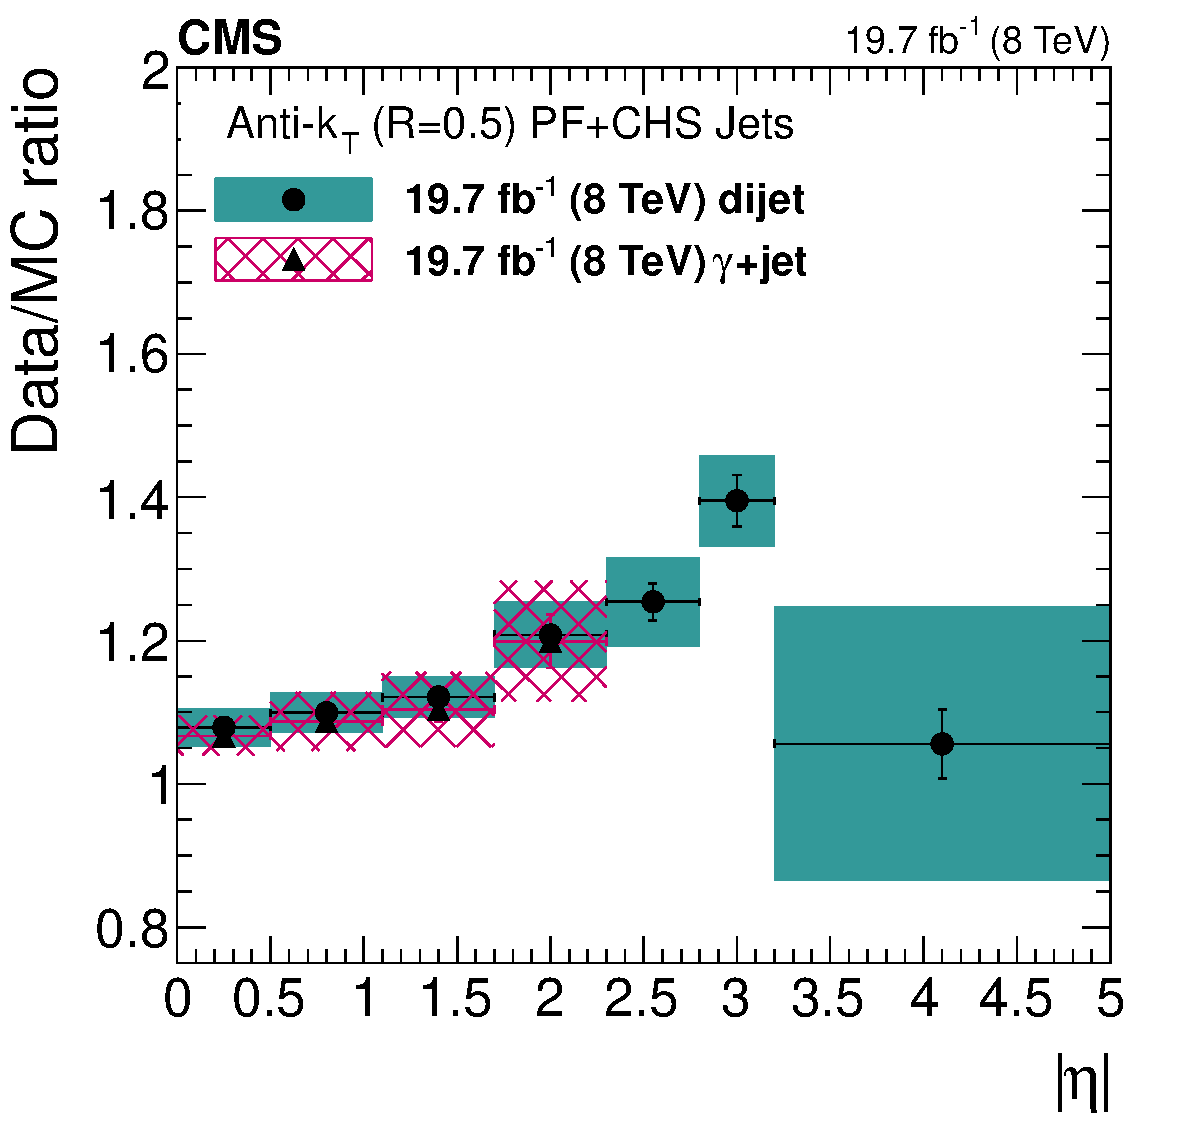
\includegraphics[width=0.45\textwidth]{\chsix/resolution-ak5chs-eta.pdf}}
%\subfigure[]{\label{fig:resolcorr_ak4chs_b}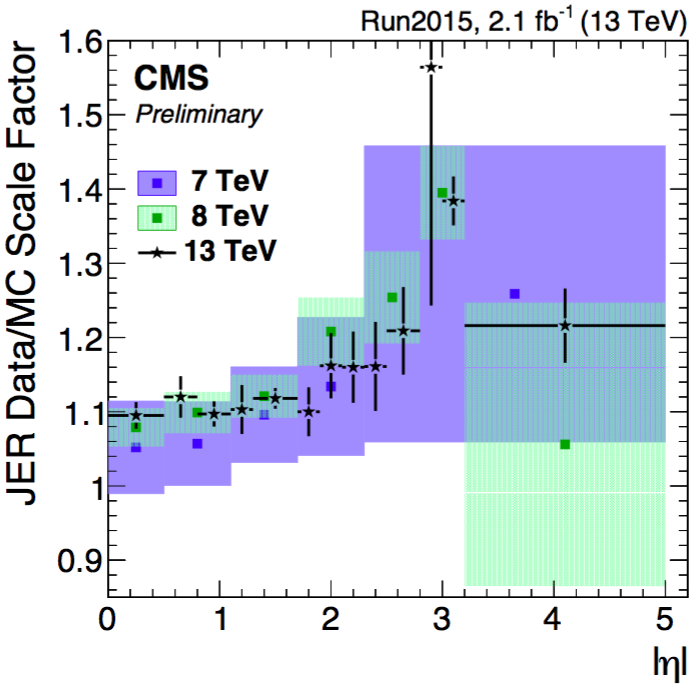
\includegraphics[width=0.45\textwidth]{\chsix/resolution-ak4chs-eta.png}}
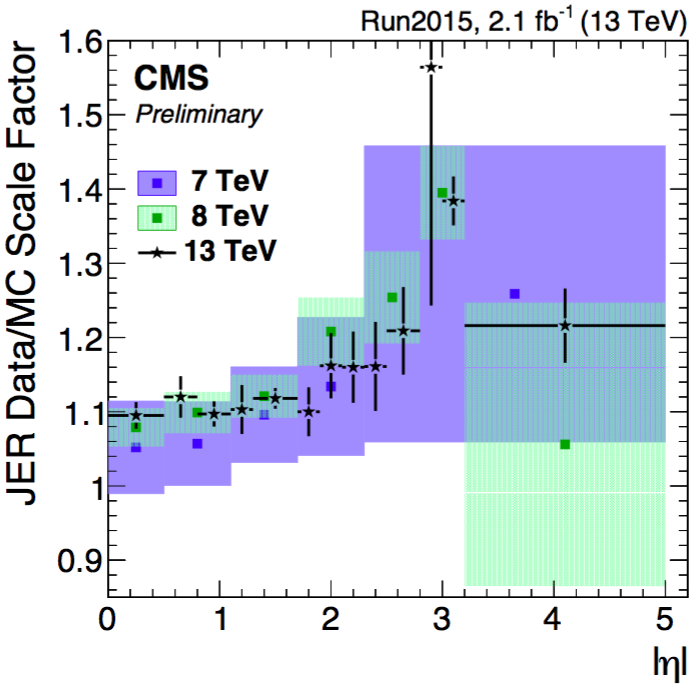
\includegraphics[width=0.45\textwidth]{\chsix/resolution-ak4chs-eta.png}
\end{center} 
\caption{Data-to-simulation scale factors for the jet \pt resolution for AK5 CHS jets as a function of $|\eta|$ determined from 8\TeV data collected in 2012, and for AK4 CHS jets in 13\TeV data collected in 2015~\cite{CMS-DP-2016-020}.}
\label{fig:resolcorr813TeV}
\end{figure}

%%%%%%%% 
\subsection{Identification of b jets}\label{subsec:bjets}
%%%%%%%%
%https://twiki.cern.ch/twiki/bin/viewauth/CMS/BtagPOG
%https://twiki.cern.ch/twiki/bin/viewauth/CMS/BtagRecommendation
%https://twiki.cern.ch/twiki/bin/viewauth/CMS/BtagRecommendation74X
%https://twiki.cern.ch/twiki/bin/viewauth/CMS/BtagRecommendation53XReReco
%https://twiki.cern.ch/twiki/bin/view/CMSPublic/PhysicsResultsBTV

The identification of jets originating from b quarks (``b jets'') is one of the key ingredients of the analysis described in this work, which aims at isolating events of new physics with H bosons decaying to $\bbbar$. The ability to identify b jets (``b tagging'') plays a crucial role in reducing background coming from processes involving jets from gluons and light-flavor quarks (u, d, s), and from c quark fragmentation.

Identifying b jets relies on the properties of the weak decay and fragmentation of the b hadrons formed from the original b quarks. The most important property is the relatively long lifetime of b hadrons of about 1.5\unit{ps} ($c\tau \equiv 450\mu m$) corresponding to a flight distance that is observable with high resolution tracking detectors. A b hadron with $\pt = 50\GeV$ propagates, on average, over almost half a centimetre ($Lc \sim \gamma\tau$) before decaying. As shown in Fig.~\ref{fig:bjet}, this leads to secondary vertices displaced from the primary event vertex and charged particle tracks incompatible with the primary vertex with sizeable impact parameter. In addition, b hadrons have a large mass and large multiplicity of charged particles in the final state (about five charged particles on average per b-hadron decay). Because of the hard b-fragmentation function, the b hadron in a b jet carries a large fraction of the jet energy. Since b and c hadrons may decay semileptonically, in about 20\% (per lepton species) of the cases an electron or muon is produced inside a b jet, if both direct and cascade decays are taken into account.

\begin{figure}[!htb]
 \begin{center}
  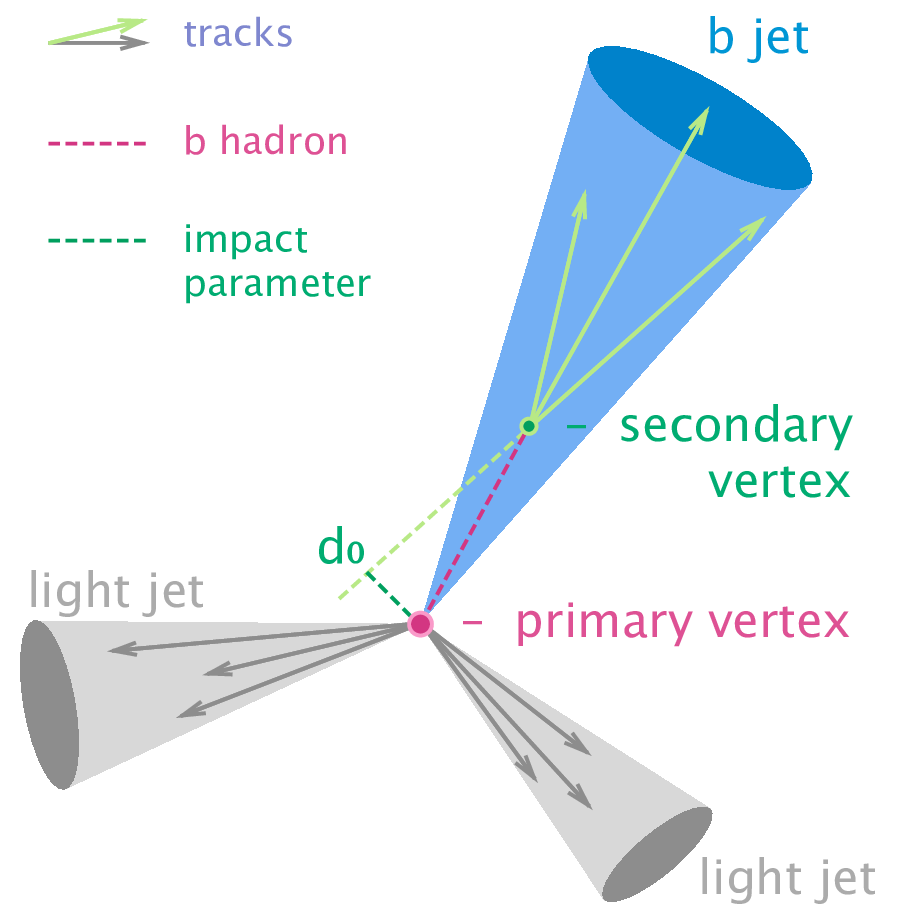
\includegraphics[width=0.5\textwidth]{\chsix/B-tagging_diagram.png}
 \end{center}
 \caption{Representation of a b-hadron decay and reconstructed b jet in the transverse plane.}
 \label{fig:bjet}
\end{figure}

A variety of algorithms have been developed in CMS~\cite{Chatrchyan:2012jua} that, starting from jets and charged tracks, identify b jets exploiting the b-hadron properties described above.
%These algorithms use low-level physics objects, mainly jets and charged tracks.
Only the tracking detectors offer the spatial resolution needed to measure the properties of b-hadron decays such as their long flight path. Efficient track reconstruction, and in particular precise spatial reconstruction close to the interaction point, is thus the key ingredient. 
Some of these algorithms use just a single observable, while others combine several of these objects to achieve a higher discrimination power. Each of these algorithms yields a single discriminator value for each jet. The minimum thresholds on these discriminators define loose (``L''), medium (``M''), and tight (``T'') operating points with a misidentification probability for light-flavor jets of 10\%, 1\%, and 0.1\%, respectively, at an average jet \pt of about 80\GeV.

The jets used for b tagging are reconstructed with the PF algorithm and calibrated as described in Section~\ref{subsec:jetsreco}. A sample of well-reconstructed tracks of high purity inside the jet is selected as input to each of the b-tagging methods. In addition to the selection applied in the iterative tracking procedure described in Section~\ref{subsec:tracks}, specific requirements are imposed:

\begin{itemize}
\item the fraction of misreconstructed or poorly reconstructed tracks is reduced by requiring $\pt >1\GeV$;
\item at least 8 tracker hits (including pixel) must be associated with the track;
\item at least 2 hits are required in the pixel system since track measurements in the innermost layers provide most of the discriminating power;
\item the normalised $\chi^2$ is required to be $< 5$ to ensure a good-quality fit;
\item the absolute value of the transverse and longitudinal impact parameter of the track must be $< 0.2$ and $< 17\unit{cm}$, respectively, to reject charged particle tracks having their origin from sources with large displacement from the primary vertex (e.g. photon conversions and nuclear interactions in the beam pipe or the first layers of the pixel detector);
\item tracks are associated to jets in a cone $\Delta R < 0.3$ around the jet axis, where the jet axis is defined by the primary vertex and the direction of the jet momentum;
\item in order to reject tracks from pileup the distance to the jet axis, defined as the distance of closest approach of the track to the axis, is required to be $< 700\mum$;
\item the point of closest approach between the track trajectory and the jet axis, must be within 5\unit{cm} of the primary vertex.
\end{itemize}

Two algorithms for reconstructing secondary vertices are exploited. For the first algorithm, the tracks associated to jets and fulfilling the above selection requirements are used in the \textit{adaptive vertex reconstruction} (AVR) algorithm~\cite{Waltenberger:1166320}, based on the adaptive vertex fitter described in Section~\ref{subsec:tracks}. This is the secondary vertex reconstruction algorithm used for b-tagging methods in CMS during Run~1. A number of selection criteria are applied to remove vertices that are less likely to originate from a b-hadron decay. 

\begin{itemize}
\item at least 2 tracks must be associated to the secondary vertex;
\item the fraction of tracks shared with the primary vertex is required to be $< 65\%$;
\item the distance between the primary vertex and the secondary vertex in the transverse plane, the 2D flight distance, must be in the range 0.1--25\mm;
\item the 2D flight distance divided by its uncertainty or so-called 2D flight distance significance has to be $> 3$;
\item the invariant mass of charged particles associated to the vertex is required to be $< 6.5\GeV$ and not compatible with the mass of the $K^0_S$ hadron in a window of 50\MeV;
\item the angular distance $\Delta R$ between the jet axis and the secondary vertex flight direction is required to be less than the jet distance parameter;
\end{itemize}

In contrast to the AVR algorithm, the \textit{inclusive vertex finder} (IVF)~\cite{Khachatryan:2011wq} is not seeded from tracks associated to the reconstructed jets. The IVF algorithm uses as input the collection of reconstructed tracks in the event and looser quality criteria are applied. The selected tracks are then used to identify clusters of nearby tracks based on their minimum distance and the angles between them. The clusters are fit with the adaptive vertex fitter and a cleaning procedure is applied. At this stage, tracks can appear in multiple vertices and therefore, one of the vertices is removed based on the number of shared tracks and distance between the vertex and another one. Furthermore, tracks in the secondary vertex compatible with the primary vertex are removed. When there are at least 2 tracks associated to the secondary vertex after the track arbitration, the vertex is refit and selection criteria similar to the case of the AVR vertices are applied.

 The efficiency to reconstruct a secondary vertex for b (c) jets using the IVF algorithm is about 10\% (15\%) higher compared to the efficiency to reconstruct a secondary vertex with the AVR algorithm. However, for light-flavour jets the probability to find a secondary vertex also increases by about 8\%. Independently of the jet flavour, around 60\% of the jets with an AVR vertex also have an IVF vertex.\\
 
In this analysis the \textit{Combined Secondary Vertex} (CSV) b-tagging algorithm is used, which combines the information of displaced tracks with the information of secondary vertices associated to the jet.
%The CSV algorithm was further optimized and the new version is referred to as CSVv2 and it uses IVF.
This allows the algorithm to avoid limitations due to inefficiencies in the secondary vertex reconstruction. Jets are divided in three vertex-dependent exclusive categories: the presence of a reconstructed secondary vertex; at least two tracks with impact parameter significance larger than 2; none of the previous. The following set of variables with high discriminating power and low correlations are considered:

\begin{itemize}
\item the secondary vertex category;
\item the 2D flight distance significance of the secondary vertex;
\item the number of tracks in the jet;
\item the number of tracks associated to the secondary vertex;
\item the secondary vertex mass;
\item the ratio of the energy carried by tracks at the vertex with respect to all tracks in the jet;
\item the $\eta$ of the tracks at the vertex with respect to the jet axis;
\item the 2D impact-parameter significance of the first track that raises the invariant mass above the charm threshold of 1.5\GeV when subsequently summing up tracks ordered by decreasing impact parameter significance;
\item the 3D signed impact-parameter significance for each track in the jet.
\end{itemize}

Two likelihood ratios are built from these variables used to discriminate between b and c jets and between b and light-flavor jets and combined with prior weights of 0.25 and 0.75, respectively. Figure~\ref{fig:csv_813TeV_a} shows the distribution of the CSV discriminator value in a multijet sample for 8\TeV data and for simulation, for jets clustered with the AK5 algorithm.

\begin{figure}[!htb]
\begin{center}
\subfigure[]{\label{fig:csv_813TeV_a}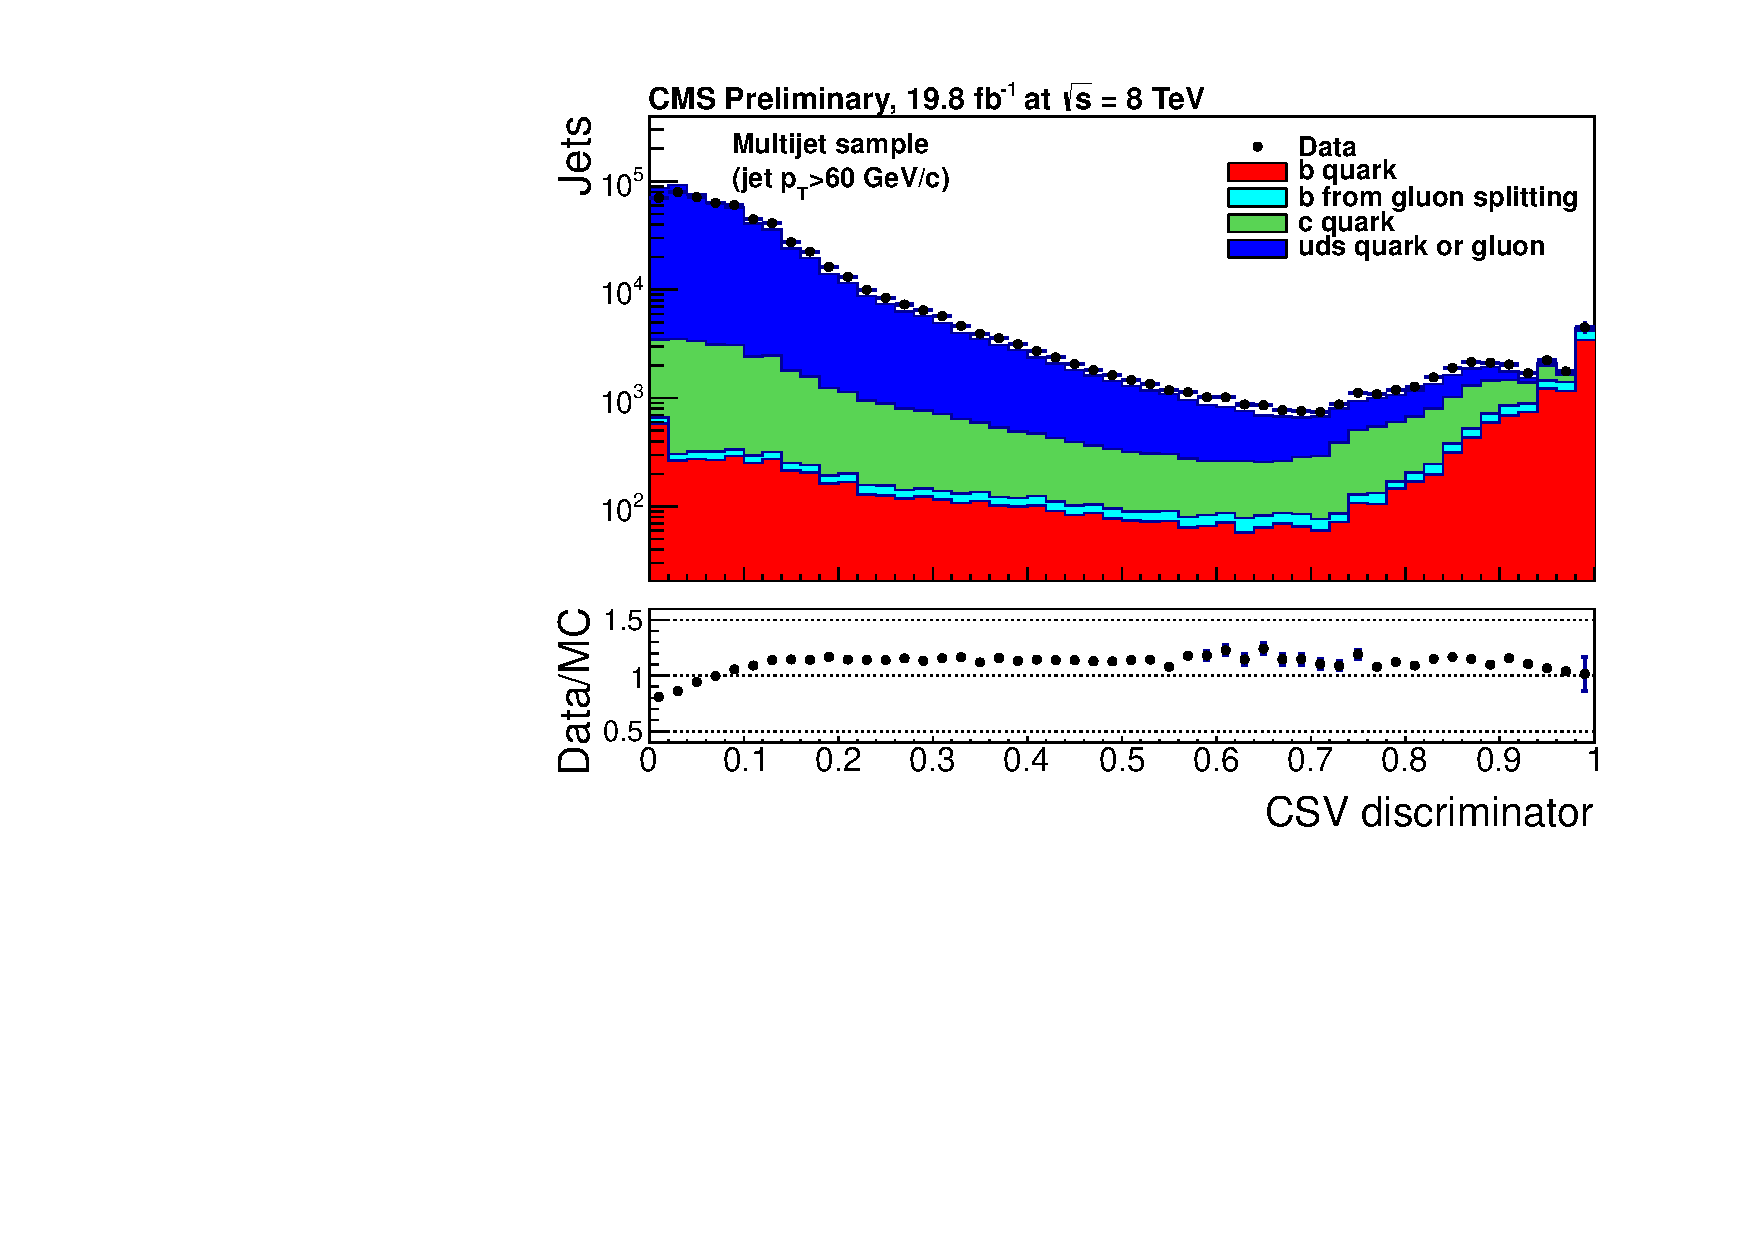
\includegraphics[width=0.45\textwidth]{\chsix/CSV-multijet-run1.pdf}}
\subfigure[]{\label{fig:csv_813TeV_b}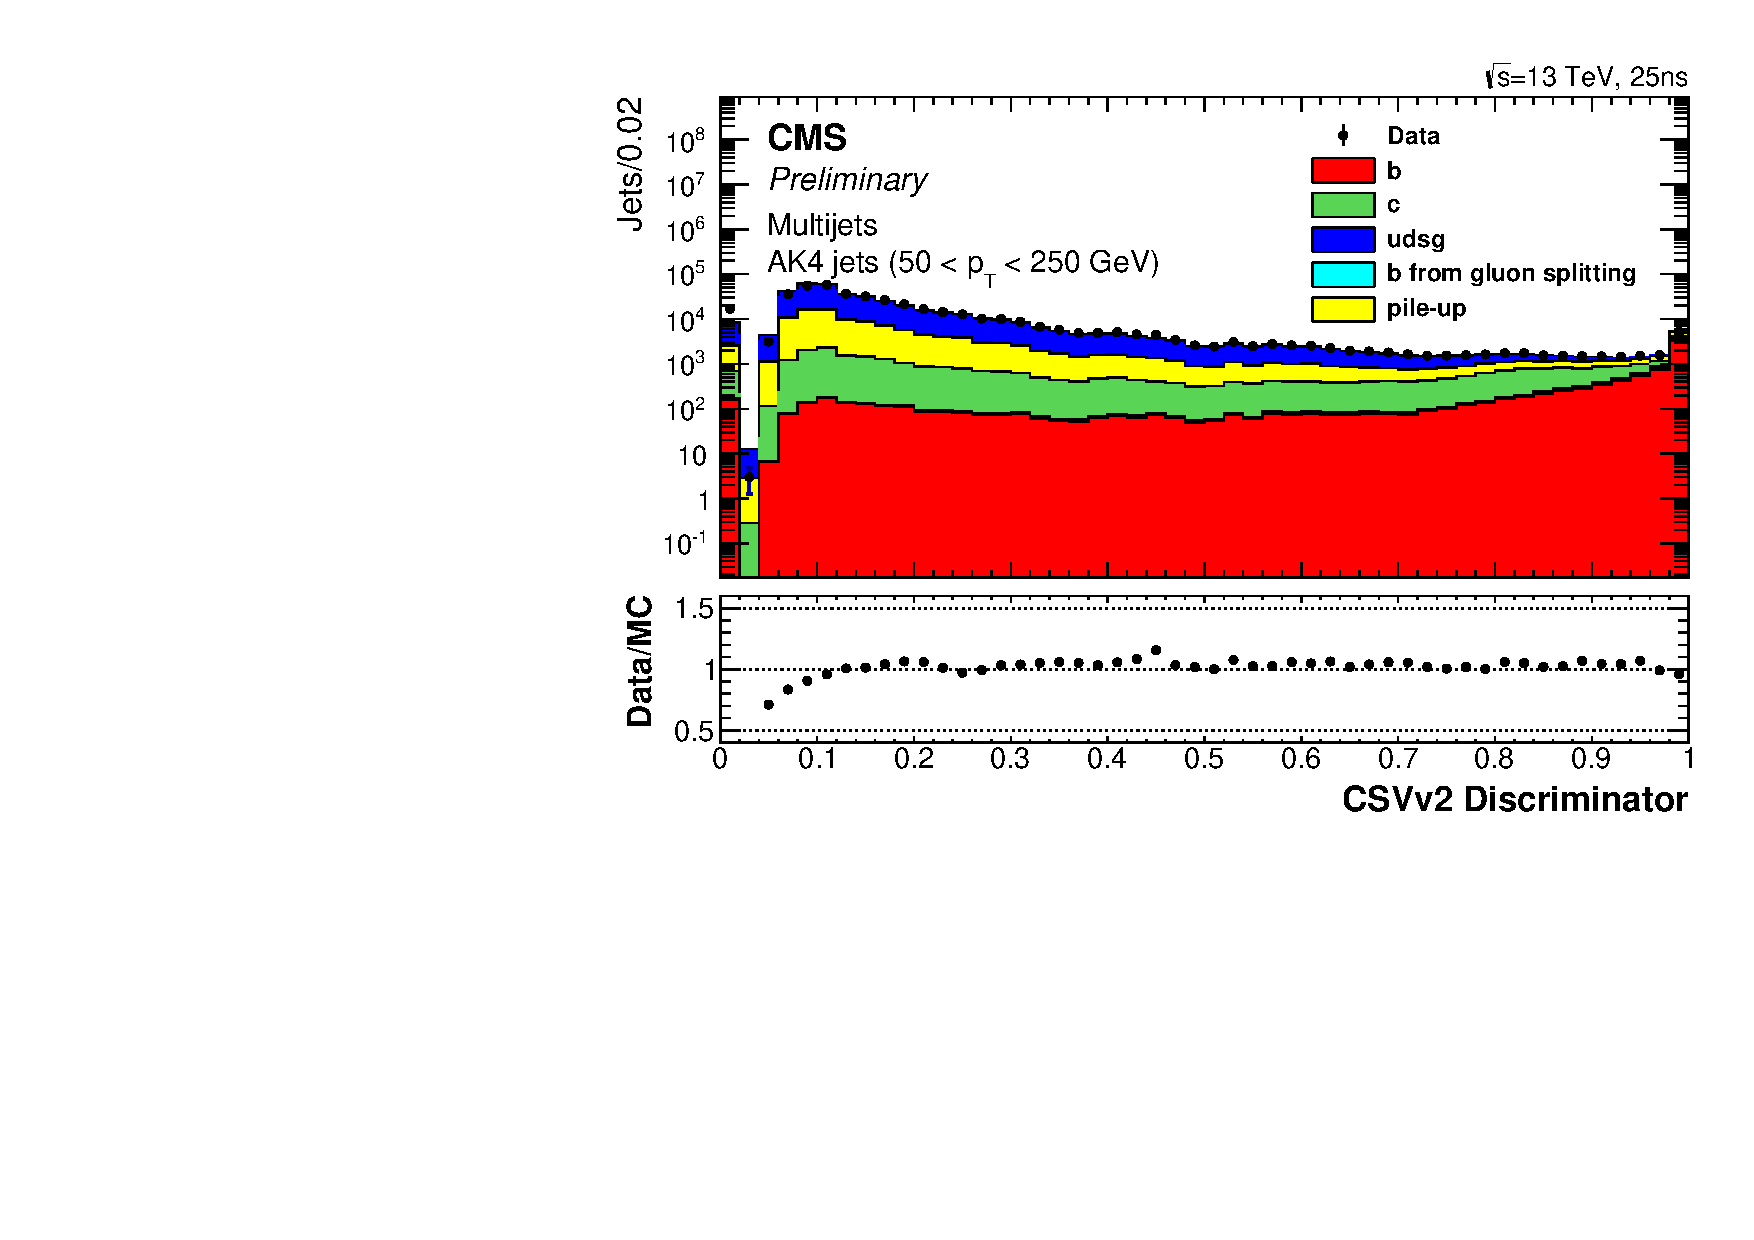
\includegraphics[width=0.45\textwidth]{\chsix/CSVv2-multijet-run2.pdf}}
\end{center} 
\caption{(a) Distribution of the CSV discriminator value in a multijet sample for data collected at 8\TeV and for simulation~\cite{CMS:BTV13001}, for jets reconstructed with the AK5 algorithm. (b) Distribution of the CSVv2 discriminator value in a multijet sample for data collected at 13\TeV and for simulation, for jets reconstructed with the AK4 algorithm~\cite{CMS-PAS-BTV-15-001}.}
\label{fig:csv_813TeV}
\end{figure}

The CSV algorithm was further optimized for Run~2 and the new version is referred to as CSV version 2 (CSVv2)~\cite{CMS-PAS-BTV-15-001}. The main differences with respect to the Run~1 version of the CSV algorithm are the different vertex reconstruction algorithm used, the number of input variables and the way those are combined. As in the previous version, the input variables are combined using a multivariate technique. However, the method previously used limited the amount of input variables since correlation between those could not be taken into account properly. In addition, the secondary vertex information is obtained with the IVF method described above. Figure~\ref{fig:csv_813TeV_b} shows the distribution of the CSVv2 discriminator value in a multijet sample for 13\TeV data and for simulation, for jets clustered with the AK4 algorithm.

The performance of the CSVv2 tagger is presented in Fig.~\ref{fig:btagalgo} as the b-jet identification efficiency versus the misidentification probability for jets in simulated \ttbar events requiring jet $\pt > 30\GeV$. A comparison is shown with the Run~1 version of the CSV algorithm trained for 8\TeV pp collisions using AK5 jets. The absolute improvement of the CSVv2 algorithm with respect to the CSV is of the order of 2 to 4\% in b-jet identification efficiency when comparing at the same misidentification probability for light-flavour jets. The improvement of using IVF vertices with respect to using AVR vertices in the CSVv2 algorithm is of the order of 1 to 2\%.\\
%For light-flavour jets, the absolute efficiency improves by about 4\% with respect to the CSVv2 algorithm.

\begin{figure}[!htb]
 \begin{center}
  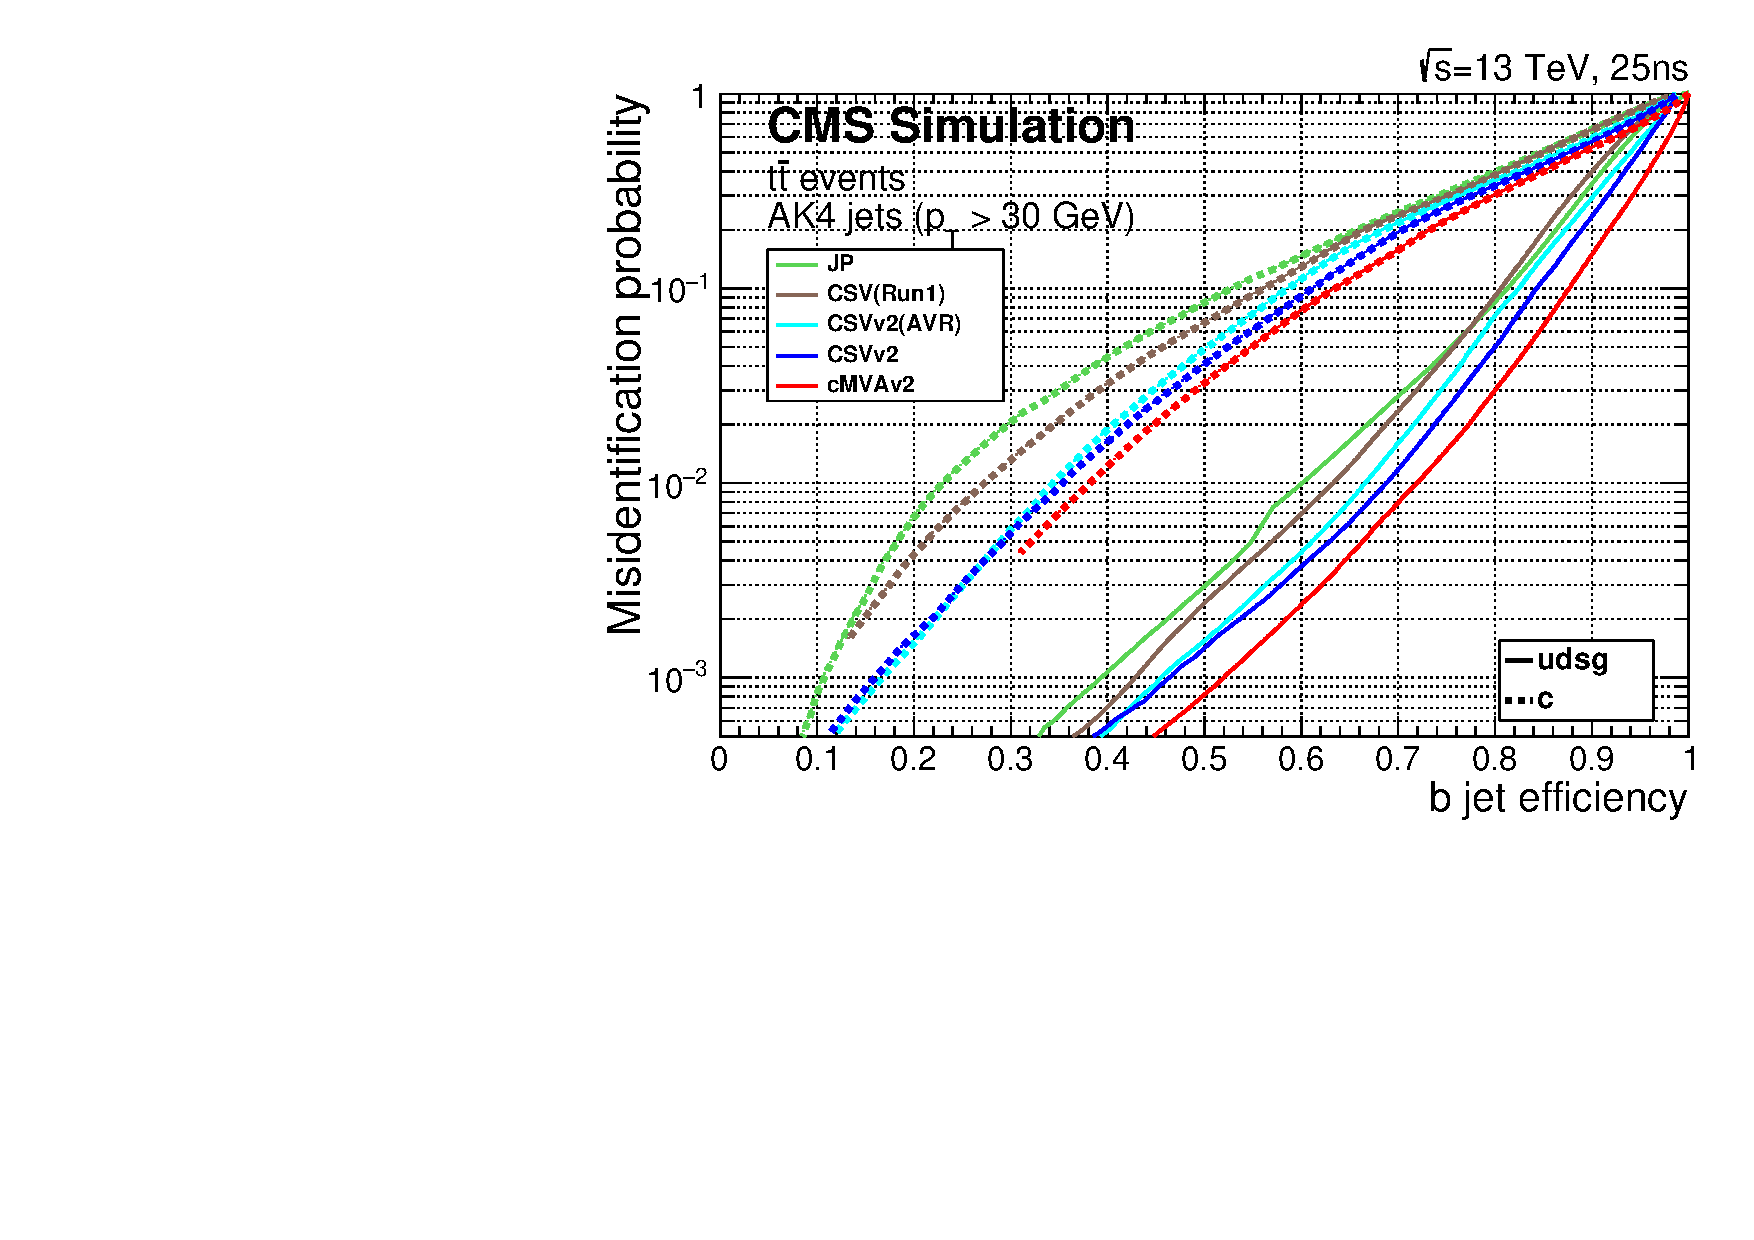
\includegraphics[width=0.45\textwidth]{\chsix/btagalgo-ak4jets.pdf}
 \end{center}
 \caption{Performance of the CSVv2 algorithm showed as the probability for non-b jets to be misidentified as b jet as a function of the efficiency to correctly identify as b jets. The improvement of this algorithm with respect to the Run~1 version is also shown~\cite{CMS-PAS-BTV-15-001}.}
 \label{fig:btagalgo}
\end{figure}

The value of the discriminator threshold for the b-tagging algorithms used in this analysis and the corresponding efficiencies are presented in Table~\ref{tab:btagwp}.
In this analysis the medium working point is used to identify and reject \ttbar events where a real b jet is expected in addition to the large-cone jet used to reconstruct the $\PV\to\qqbarpr$ or $\PH\to\bbbar$ candidate, representing instead the signal. The same b-tagging algorithm but together with the loose working point is used to identify whether the CA8 jet comes from a H boson decaying into bottom quarks, as described in Section~\ref{sec:htagging}.

\begin{table}[!htb]
\centering
\caption{B taggers and discriminator threshold used in CMS for Run~1 and Run~2 and corresponding efficiency for b jets with $\pt > 30\GeV$ in simulated \ttbar events. }
\resizebox{\textwidth}{!}{
\begin{tabular}{ l | c | c | c}
Algorithm & Operating point & Discriminator value & B-tagging efficiency (\%)\\ 
\hline
\hline
\multirow{3}{*}{CSV (Run 1)} & CSVL & 0.244 & 80\\
 & CSVM & 0.679 &  64\\
 & CSVT & 0.898 & 42\\
\multirow{3}{*}{CSVv2 (Run 2)} & CSVv2L & 0.460 & 83\\
 & CSVv2M & 0.800 & 69\\
 & CSVvsT & 0.935 & 49\\
\end{tabular}}
\label{tab:btagwp}
\end{table}

The mismodelling of the b-tagging variables in simulation is taken into account by reweighting simulation event-by-event with the ratio of the b-tagging efficiency in data and simulation, determined in a sample enriched with b jets and depending on the jet \pt and $\eta$. The correction factors as a function of the b-jet \pt  are shown in Fig.~\ref{fig:btag_sfb_a} and~\ref{fig:btag_sfb_b} for the CSVM and CSVv2M operating points respectively, as measured in 8 and 13\TeV data. In a similar way, correction factors are also derived and applied to correct the misidentification probability in simulation. These factors are shown in Fig.~\ref{fig:btag_sfl_a} and~\ref{fig:btag_sfl_b} as a function of the jet \pt for the CSVM and CSVv2M operating points.
%The average scale factors are reported in Table~\ref{tab:btagwp} for the two b tagging algorithms used in this analysis. The average values of the correction factors $SF_\mathrm{b}$ are 0.95 and 0.93 for the CSVM, and CSVv2M algorithms, respectively. While average values of 1.17 for are obtained for $SF_\mathrm{light}$ for the CSVM algorithm.

\begin{figure}[!htb]
\begin{center}
\subfigure[]{\label{fig:btag_sfb_a}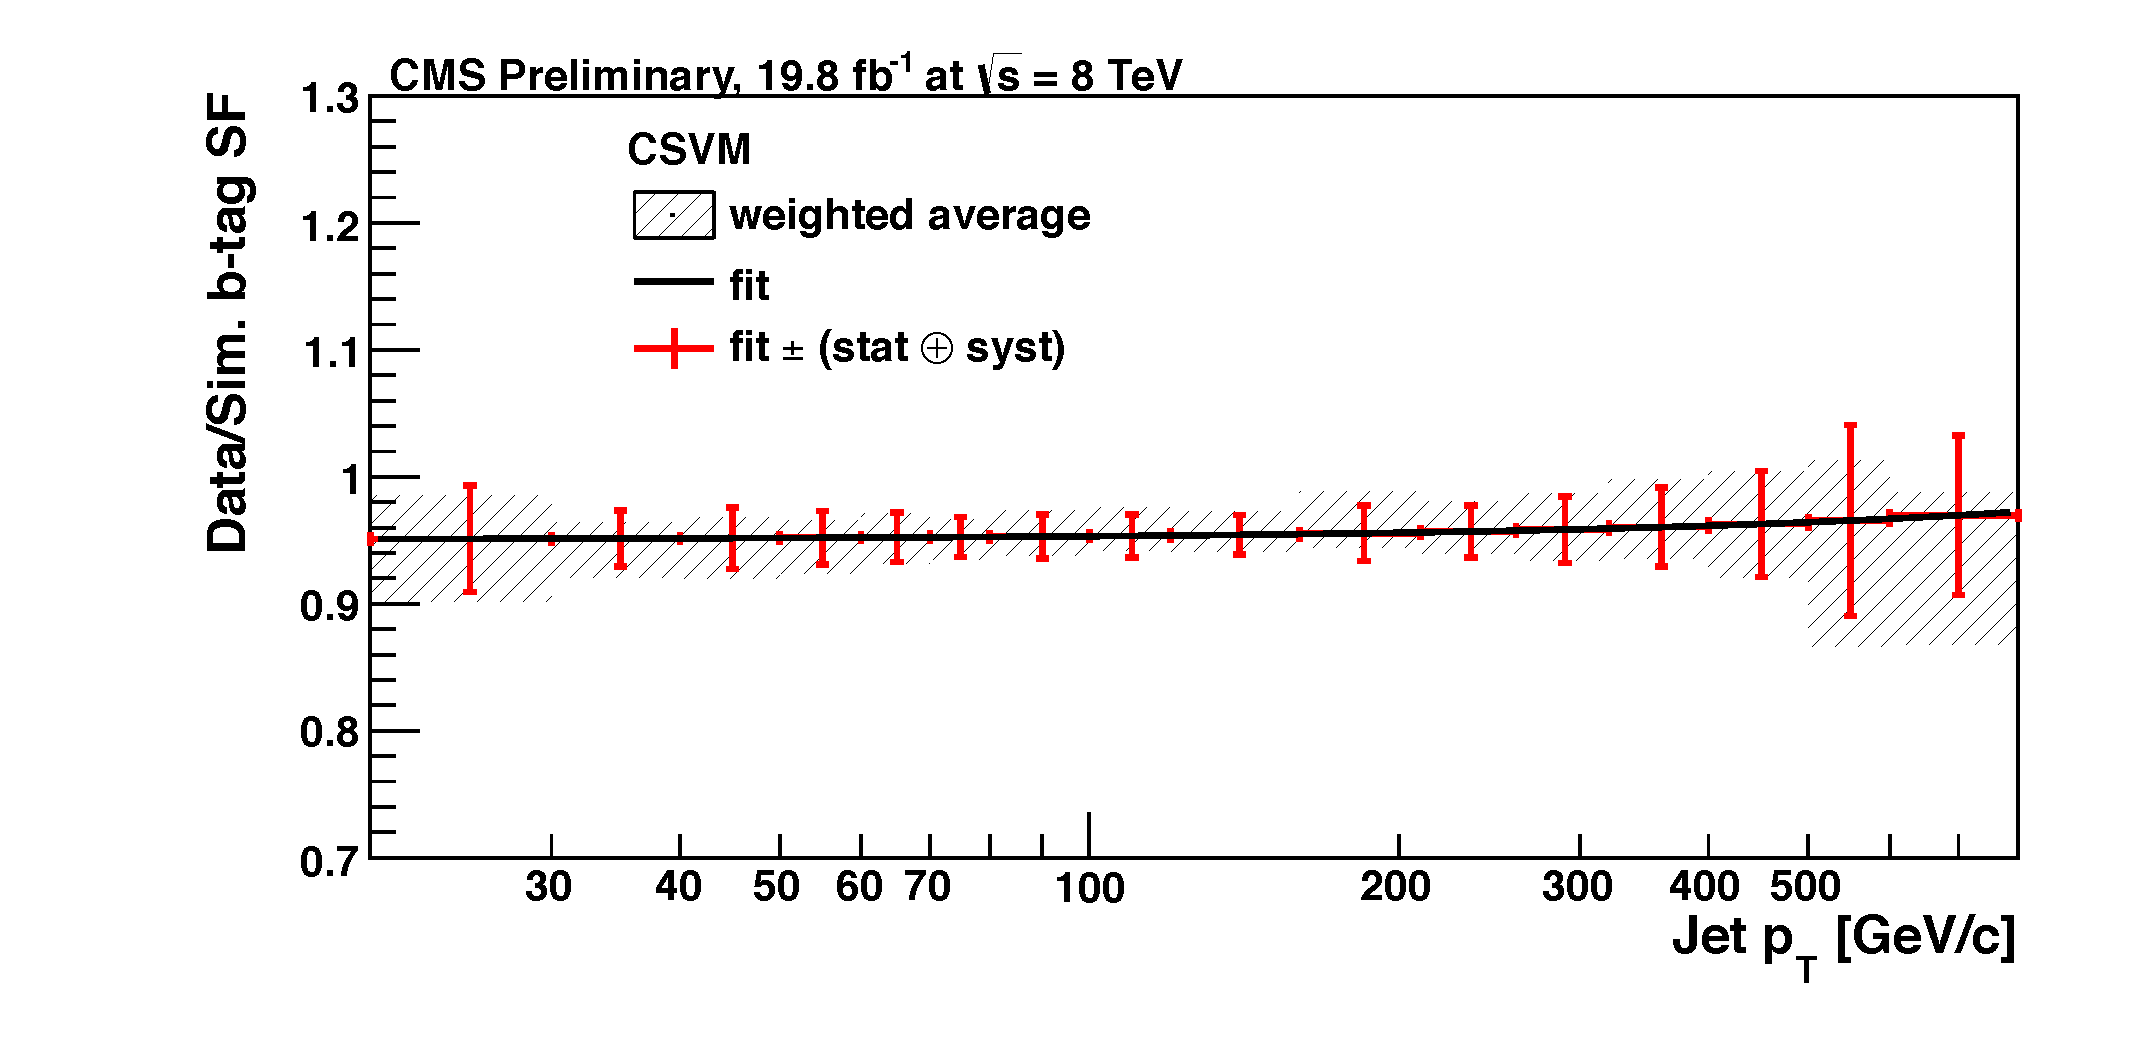
\includegraphics[width=0.45\textwidth]{\chsix/btag-sfb-pt-csvm-run1.pdf}}
\subfigure[]{\label{fig:btag_sfb_b}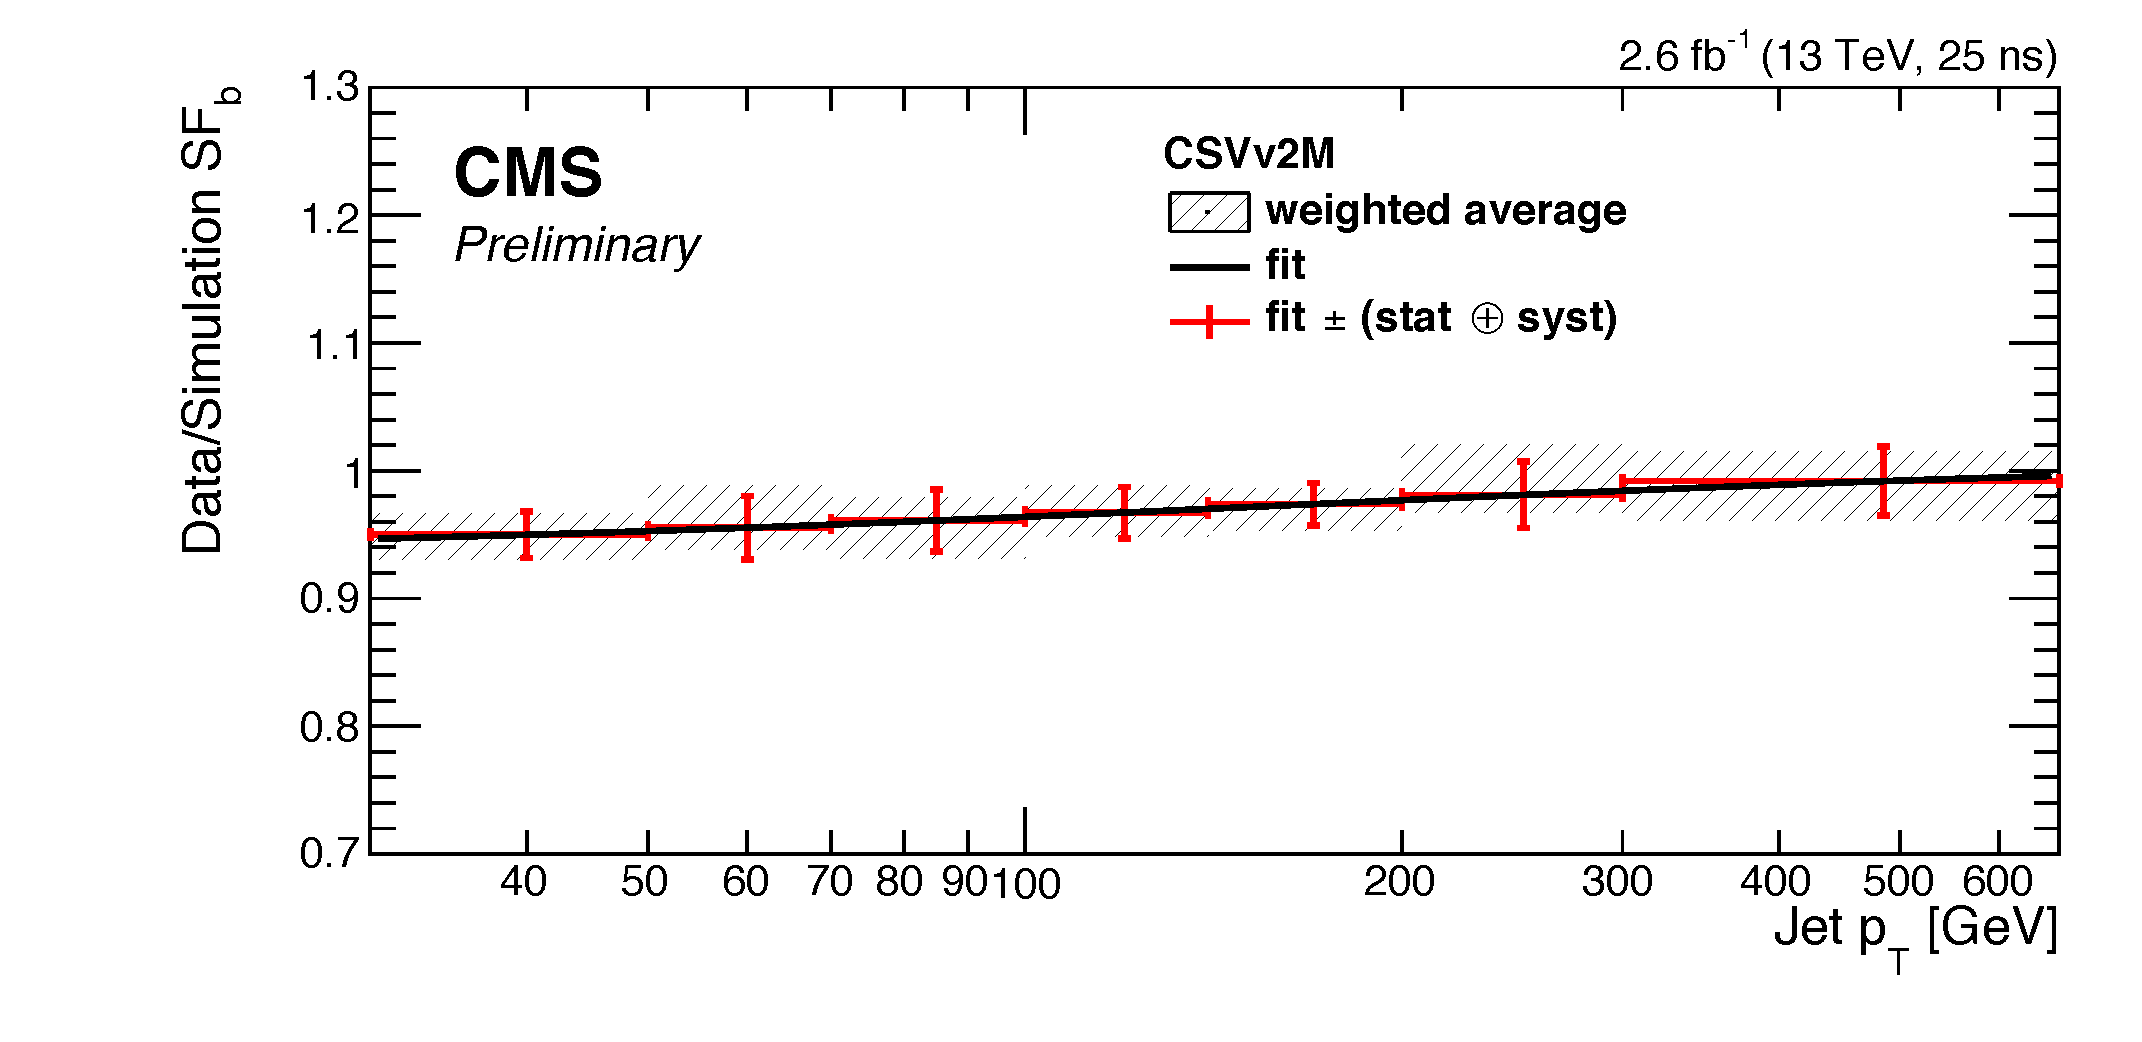
\includegraphics[width=0.45\textwidth]{\chsix/btag-sfb-pt-csvv2m-run2.pdf}}
\end{center} 
\caption{Data-to-simulation correction factors for the b-tagging efficiency for the CSVM (a) and CSVv2M (b) algorithms as a function of the b-jet \pt as measured in 8 and 13\TeV data~\cite{CMS:BTV13001,CMS-PAS-BTV-15-001}.}
\label{fig:btag_sfb}
\end{figure}

\begin{figure}[!htb]
\begin{center}
\subfigure[]{\label{fig:btag_sfl_a}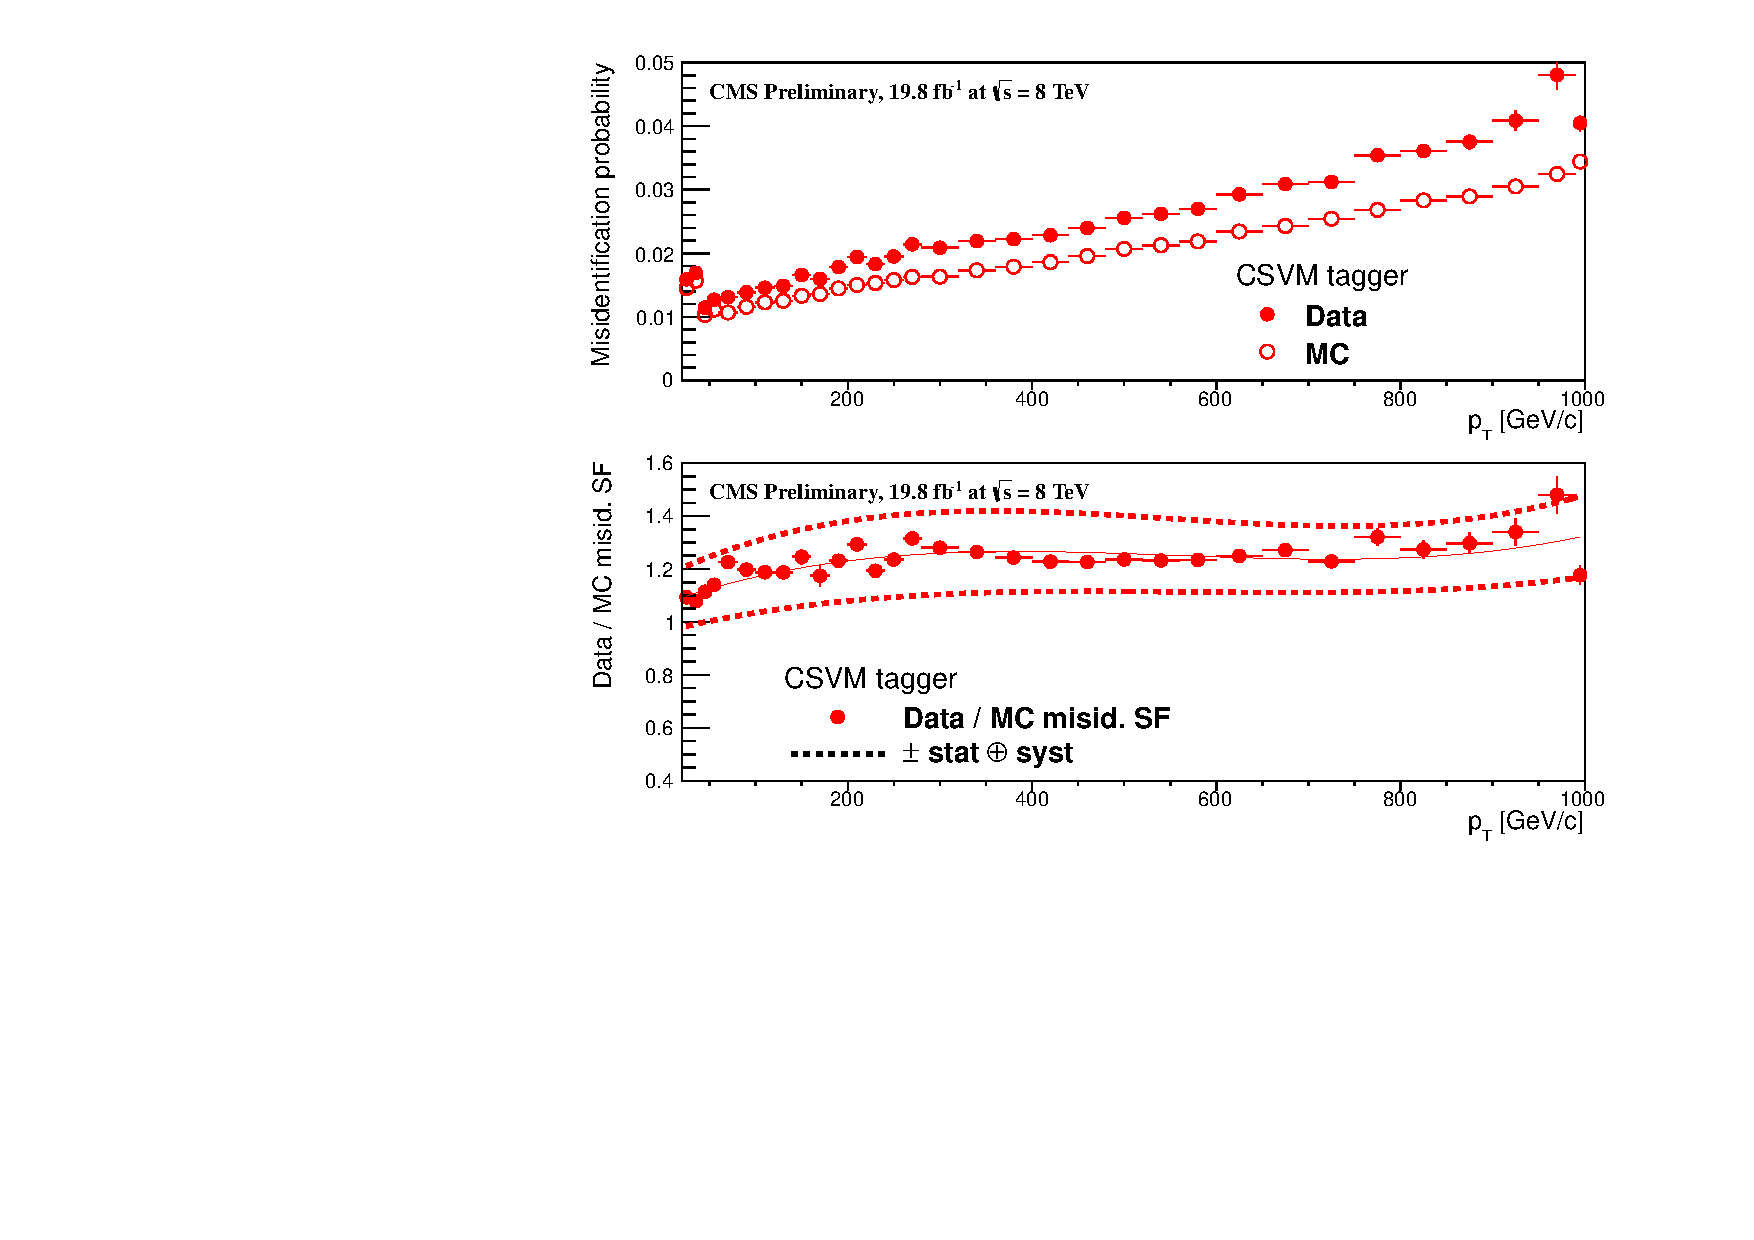
\includegraphics[width=0.45\textwidth]{\chsix/btag-SFlight-csvm-run1.pdf}}
\subfigure[]{\label{fig:btag_sfl_b}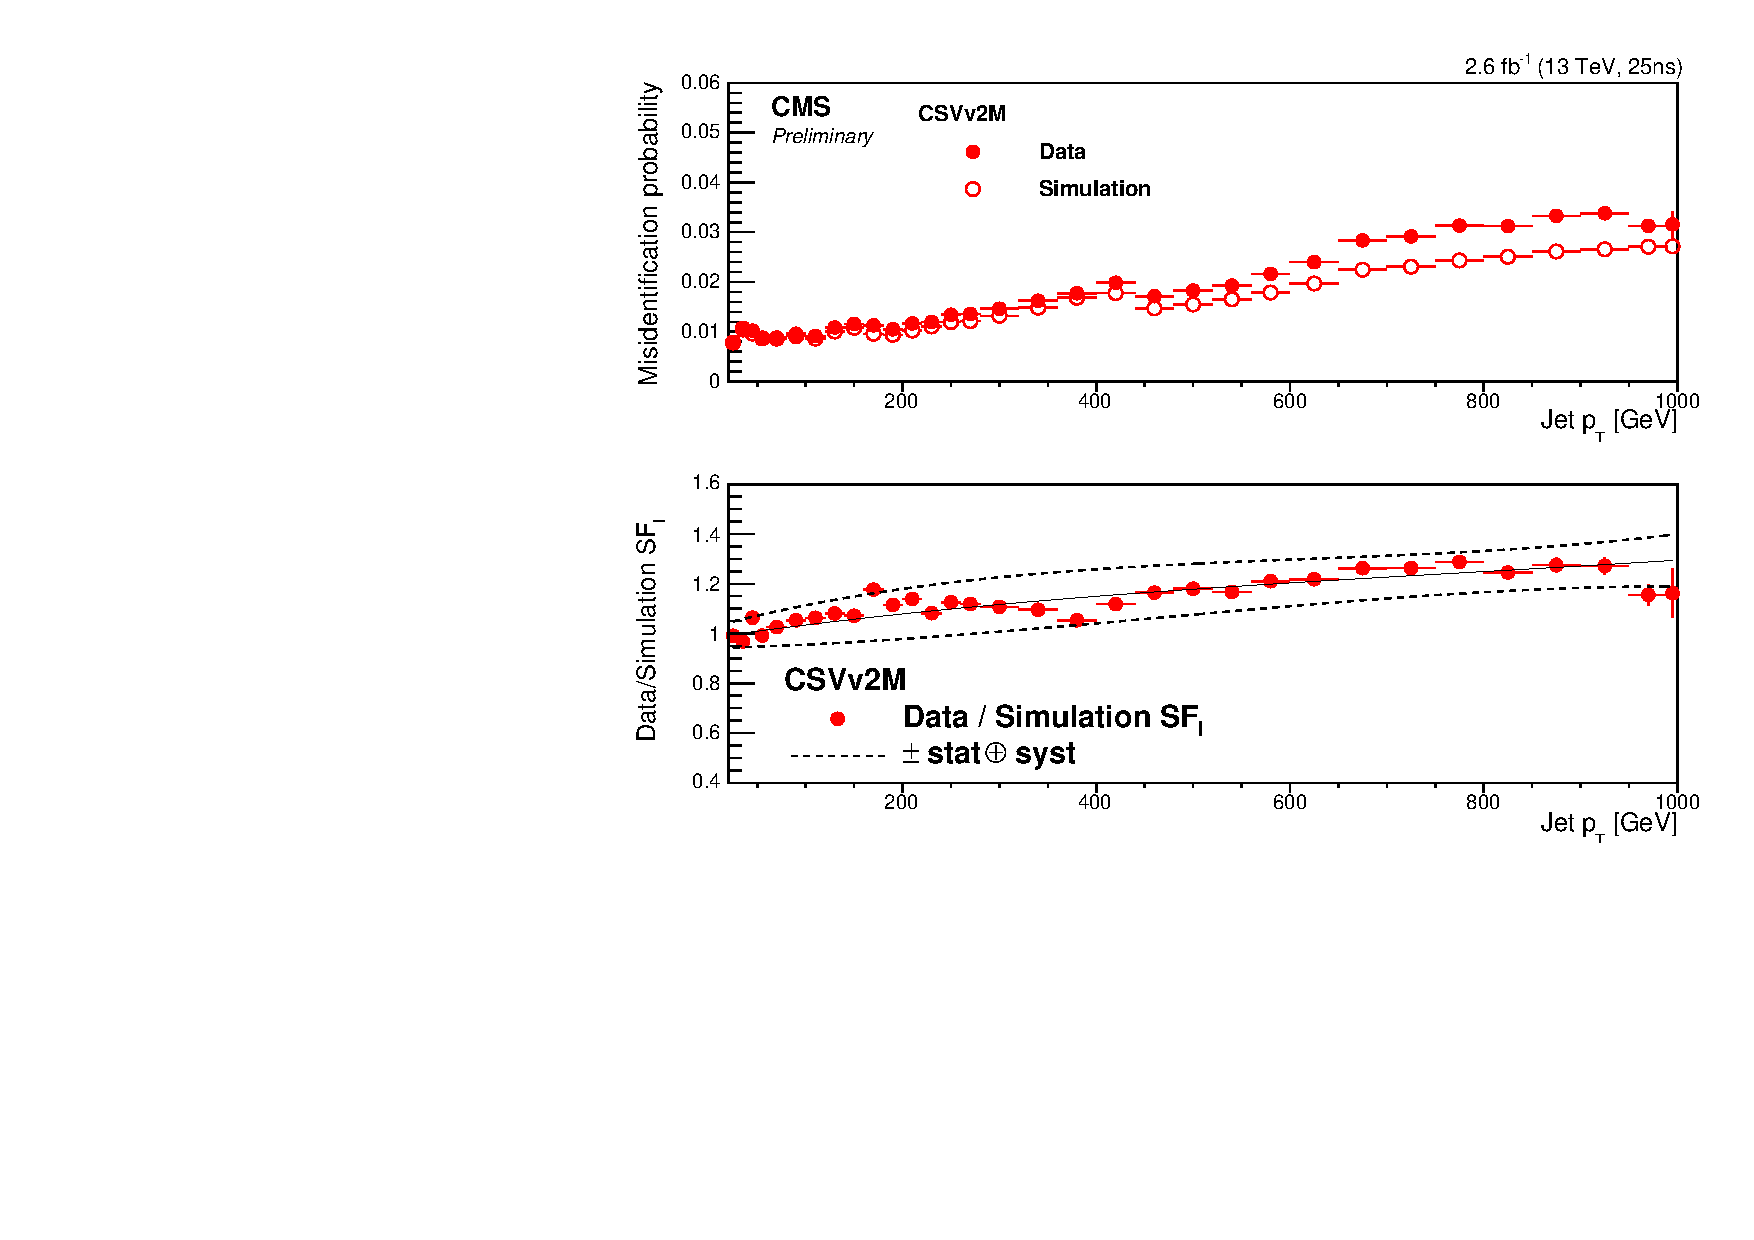
\includegraphics[width=0.45\textwidth]{\chsix/btag-SFlight-csvv2m-run2.pdf}}
\end{center} 
\caption{Data-to-simulation correction factors for the misidentification probability for the CSVM (a) and CSVv2M (b) algorithms as a function of the jet \pt as measured in 8 and 13\TeV data~\cite{CMS:BTV13001,CMS-PAS-BTV-15-001}.}
\label{fig:btag_sfl}
\end{figure}